\documentclass[11pt]{article}
\usepackage{amsfonts,amsmath,amssymb,amsthm}
\usepackage{graphicx,psfrag,epsf}
\usepackage{enumerate}
\usepackage{url} % not crucial - just used below for the URL
\usepackage{algorithm}
\usepackage{algpseudocode}
\usepackage{subfig}
\usepackage{authblk}
\usepackage{verbatim} %used to comment out unnecessary contents
\usepackage{helvet}
\usepackage[colorlinks=true,pagebackref,linkcolor=magenta]{hyperref}
\usepackage[sort&compress,comma,square,numbers]{natbib}
\usepackage{fullpage,fancyhdr}
\renewcommand{\familydefault}{\sfdefault}
\usepackage{color} %used to highlight changes
\usepackage{paralist}
\usepackage{lineno}
% \usepackage{todonotes}
\usepackage[font=small,labelfont=bf]{caption}
\usepackage[final,authormarkup=none]{changes}
\newcommand{\note}[2][]{\added[#1,remark={#2}]{}}
\definecolor{green}{rgb}{0.1840,0.4362,0.1003} 
% \usepackage[nottoc,numbib]{tocbibind}
% \usepackage{flushend}


%better toc
% \usepackage{tocloft}
% \setlength\cftparskip{-1pt}
% \setlength\cftbeforesecskip{2pt}
% \setlength\cftaftertoctitleskip{4pt}


\pagestyle{fancy}
% \oddsidemargin=-0.5in
% \evensidemargin=-0.5in
\textwidth=6.5in
\headwidth=6.5in
\textheight=9.0in
\headheight=0.0pt
\topmargin=0.0in
\headsep=0.0in
\renewcommand{\headrulewidth}{0pt}

\setlength{\parindent}{0em}
\setlength{\parskip}{0.7em}

% % DON'T change margins - should be 1 inch all around.
% \addtolength{\oddsidemargin}{-.5in}%
% \addtolength{\evensidemargin}{-.5in}%
% \addtolength{\textwidth}{1in}%
% \addtolength{\textheight}{-.3in}%
% \addtolength{\topmargin}{-.8in}%


%\providecommand{\sct}[1]{{\sc \texttt{#1}}}
\providecommand{\sct}[1]{{\normalfont\textsc{#1}}}
\providecommand{\mt}[1]{\widetilde{#1}}
\providecommand{\mb}[1]{\boldsymbol{#1}}
\providecommand{\mc}[1]{\mathcal{#1}}
\newcommand{\Real}{\mathbb{R}}
\newcommand{\G}{c}
\newcommand{\K}{\mathcal{K}}
\newcommand{\LL}{\mathcal{L}}
\newcommand{\Migraine}{\sct{Migraine}}
\newcommand{\mtg}{\sct{m2g}}
\newcommand{\T}{^{\ensuremath{\mathsf{T}}}}           % transpose
\newcommand{\Linefor}[2]{%
    \State \algorithmicfor\ {#1}\ \algorithmicdo\ {#2} \algorithmicend\ \algorithmicfor%
}
\newcommand{\Lineif}[2]{%
    \State \algorithmicif\ {#1}\ \algorithmicdo\ {#2} \algorithmicend\ \algorithmicif%
}\newcommand{\subfigimg}[3][,]{%
  \setbox1=\hbox{\includegraphics[#1]{#3}}% Store image in box
  \leavevmode\rlap{\usebox1}% Print image
  \rlap{\hspace*{12pt}\raisebox{\dimexpr\ht1-0\baselineskip}{#2}}% Print label
  \phantom{\usebox1}% Insert appropriate spcing
}

\newcommand{\Mgc}{\sct{Mgc}}
\newcommand{\Mgcp}{\sct{Mgc$_P$}}
\newcommand{\Mgcd}{\sct{Mgc$_D$}}
\newcommand{\Mgcm}{\sct{Mgc$_M$}}
\newcommand{\Hhg}{\sct{Hhg}}
\newcommand{\Dcorr}{\sct{Dcorr}}
\newcommand{\Mcorr}{\sct{Mcorr}}
\newcommand{\Mantel}{\sct{Mantel}}

\newcommand{\website}{\url{https://github.com/jovo/MGC/}}

\newcommand{\jv}[1]{{\note{jv: #1}}}
\newcommand{\jovo}[1]{{\note{jv: #1}}}
\newcommand{\cs}[1]{{\note{cs: #1}}}

\newcommand{\mbx}{\ensuremath{\mb{x}}}
\newcommand{\mby}{\ensuremath{\mb{y}}}
\newcommand{\rto}{\leftarrow}
\newcommand{\argmax}{\operatornamewithlimits{argmax}}
\newcommand{\argmin}{\operatornamewithlimits{argmin}}


% \linenumbers



%environment
\newtheorem{thm}{Theorem}
\newtheorem{appThm}{Theorem}
\setcounter{appThm}{0}
\newtheorem{lem}{Lemma}
\newtheorem{appLem}{Lemma}
\setcounter{appLem}{0}
\newtheorem{cor}{Corollary}
\newtheorem*{defi*}{Properties}
\newtheorem{asn}{Assumption}
\newcommand*\mean[1]{\bar{#1}}

\renewcommand{\algorithmicrequire}{\textbf{Input:}}
\renewcommand{\algorithmicensure}{\textbf{Output:}}

\begin{document}

\def\spacingset#1{\renewcommand{\baselinestretch}%
{#1}\small\normalsize} \spacingset{1}

% \title{\bf Dependence Discovery from Multimodal Data via  Multiscale Generalized Correlation}
\title{\bf Revealing the Structure of Dependency Between Multiple Data Modalities}
 % Datasets via  Multiscale Generalized Correlation}
\author[1,2]{Cencheng Shen} %\thanks{cshen@temple.edu}}
\author[2,3]{Carey E. Priebe}% \thanks{cep@jhu.edu}}
\author[4]{Mauro Maggioni}%\thanks{mauro.maggioni@duke.edu}}
\author[2,5]{Joshua T. Vogelstein\thanks{jovo@jhu.edu}}
\affil[1]{Department of Statistics, Temple University}
\affil[1]{Center for Imaging Science, Johns Hopkins University}
\affil[3]{Department of Applied Mathematics and Statistics, Johns Hopkins University}
\affil[4]{Department of Mathematics, Duke University}
\affil[5]{Department of Biomedical Engineering and Institute for Computational Medicine, Johns Hopkins University}
\maketitle
\pagestyle{empty}

% \bigskip
\begin{abstract}
Discovering and understanding dependence between multiple  measurements is a fundamental task not just in the natural sciences, but also policy, commerce, and other domains.
Given a set of paired observations an ideal dependence test would efficiently detect dependence in both simulated and real ``dirty'' data, regardless of the nature of the dependence structure, including nonlinear,  high-dimensional, low-sample size, and structured observations, such as images and their corresponding captions.  Moreover, rather than merely providing a theoretically consistent test under all those conditions, it would also provide insight into the nature of the dependence between the different modalities.  
No existing test satisfies all of these properties.
We propose a dependence test statistic called ``Multiscale Generalized Correlation'' (\Mgc), by combining the ideas of generalized correlation coefficient with multiscale neighborhoods.
Our key insight is that if the two different modalities are dependent, then local distances within one modality (images) should correlate with local distances within the other modality (captions).  
We demonstrate that \Mgc~has all of the above properties via simulation and theory.
We then apply \Mgc~in several real applications to detect the presence and nature  of dependence between: (i)  brain activity and personality, (ii) brain shape and disorder, and (iii) brain connectivity and creativity; as well as demonstrate that \Mgc~does not inflate non-existent dependence between brain activity and spurious stimulation.  
\Mgc~is therefore poised to be useful in a wide variety of applications, requiring only data and a dissimilarity function for both measurement types.  Both MATLAB and R code are provided here: \website.
\end{abstract}


\noindent%
{\it Keywords: testing independence, distance correlation, k-nearest-neighbor, kernel test, permutation test}
% \vfill

% \clearpage
\setcounter{tocdepth}{2}% paragraphs and above
% {\small\tableofcontents}
% \addtocontents{toc}{\vspace{-3\baselineskip}}
% \listofchanges[style=list]



% submitting to science, we get 320 for content
% total: 455, need to remove >100 lines, almost entirely from results.


% \newpage
\spacingset{1.45}


% 73 lines; target = 64
% \section{Introduction}

Detecting dependency among multiple data sets is one of the most important and fundamental tasks in computational statistics and data science.
Indeed, prior to embarking on a predictive machine-learning investigation, one might first check whether any dependence is detectable; if not, high-quality predictions will be unlikely.
The founders of statistics first highlighted the importance of this task when Pearson proposed his Product-Moment Correlation statistic in 1895 \cite{Pearson1895}.  Since then, researchers have consistently developed new and improved methods (see \cite{Reimherr2013,JosseHolmes2013} for  recent reviews and discussion).

In the era of big data, several challenges emerge as particularly prevalent and therefore, problematic.
%
First, the dependencies between different modalities of data can be highly \textbf{non-linear}.  While this has always been the case, the relative abundance of data has led to an increased demand in checking for dependence in many previously uninvestigated settings.

Second, the \textbf{dimensionality} of individual samples is growing at exponential rates, with genomics and connectomics data, for example, often accruing millions or billions of dimensions per data point. At the same time, the \textbf{sample sizes} are not increasing proportionally, meaning that we often have datasets with very high-dimensions and relatively low sample size.
%
Third, the data are often \textbf{complicated}: networks, shapes, questionnaires, semi-structured text are all typical examples.
% this could improve.  possibly elaborating upon what we mean, eg, non-euclidean.
For example, we may desire to understand whether brain shape and disease status are related, so that we can develop prognostic biomarkers to combat the deleterious efforts of degenerative neurological disorders \cite{ParkEtAl2008}.
%
%Fourth, because the acquisition of data has became so easy, and quality control still typically requires human supervision, the modern datasets often exhibit a large number of \textbf{outliers}, that is, samples with egregious errors.
%
Fourth, because we will often have a data deluge, with myriad different measurements, it is important to be able to compute the results reasonably \textbf{efficiently}.
%
Fifth, when working with big data, statistical procedures often have hyper-parameters that require tuning.  Many such procedures lack any guidance in choosing the value of those hyper-parameters, thereby requiring users of the procedures to concoct their own heuristics. It is desirable that a procedure is \textbf{adaptive}, in that it can automatically set its hyper-parameters in a valid way.
%
Finally, as alluded to above, checking for dependence is rarely the final step in the analysis.  Frequently, investigators and analysts desire more than a simple p-value, rather, they desire some insight into the nature of the \textbf{dependence structure}, which can then inform them in terms of how to proceed.
%
% Thus, dependence tests that work in non-linear, high-dimensional, low sample size, complex datasets, even in the presence of many outliers, reasonably quickly, and automatically adaptive to the data, and provide insight in addition to valid p-values, are highly desirable. Moreover, w
We desire tests that satisfy the above desiderata, both in theory as well as in extensive simulations and real data problems.
% 
% 
There are two key insights from the literature that we combine to develop our methodology that satisfies the above desiderata.  

% First, a collection of pairwise comparisons suffices to characterize a joint distribution \cite{Maa1996}.  
% Second, nonlinear manifolds can be approximated by local linear spaces \cite{Allard2012}.  Our approach, Multiscale Generalized Correlation (\Mgc), leverages and improves upon recent developments from both subdisciplines of data science.

Interpoint pairwise comparison matrices have been used for over 100 years for various statistical purposes. % \cite{Pearson1895}. 
% More recently, Maa et al. proved that collection of pairwise comparisons suffices to characterize their joint distribution \cite{Maa1996}.
% 
One of the earliest examples of using them for dependence testing comes from  Karl Pearson \cite{Pearson1895}, who created  a special case of something subsequently called a ``generalized correlation coefficient'' \cite{KendallBook}.
Generalized correlation coefficients start with $n$ pairs of observations $(\mb{x}_i,\mb{y}_i)$ for $i=1,\ldots,n$, where $\mb{x}$'s and $\mb{y}$'s both might be vectors of arbitrary dimensions, shapes, networks, etc.  And then, a comparison function is defined for each.  Specifically, let $a_{ij}=\delta_x(\mb{x}_i,\mb{x}_j)$, and let $b_{ij}=\delta_y(\mb{y}_i,\mb{y}_j)$.  
Thus, $A=\{a_{ij}\}$ and $B=\{b_{ij}\}$ are the $n \times n$ interpoint comparison matrices for $X=\{\mb{x}_{i}\}$ and $Y=\{\mb{y}_{i}\}$, respectively.  
Without loss of generality, assuming $\{a_{ij}\}$ and $\{b_{ij}\}$ have zero mean, a generalized correlation coefficient can then be written:
\begin{equation}
\label{generalCoef}
\G= \tfrac{1}{z} {\textstyle \sum_{i,j=1}^n a_{ij} b_{ij}},
\end{equation}
where $z$ is proportional to standard deviations of $A$ and $B$, that is $z=n^2\sigma_a \sigma_b$.
In words, $\G$ is the sample correlation across \emph{pairwise comparisons} between the data matrices $X$ and $Y$, rather than the individual data samples.  
% That is, if we define $A$ and $B$ as the interpoint comparison matrices for \mb{x}~and \mb{y}~respectively, then $\G$ is simply the correlation between elements of $A$ and $B$.
$\G$ has many well known special cases historically, including Pearson's  \cite{Pearson1895}, Spearman's \cite{Spearman1904},  Kendall's \cite{KendallBook}, and Mantel's correlation \cite{Mantel1967}. % which is widely used in biology and ecology.
% Three special cases of $\G$ are particularly popular for independence testing.  First, the \Mantel~coefficient \cite{Mantel1967}, a widely-used method in biology and ecology, defines $a_{ij}=||\mb{x}_i-\mb{x}_j||_{2}$.
% \Mantel, however, does not have any theoretical support for being a generally consistent test.
More recently, Maa et al. proved that collection of pairwise comparisons suffices to characterize their joint distribution \cite{Maa1996}.
In the last decade, Szekely et al. \cite{SzekelyRizzoBakirov2007} extended these results, letting $\delta_x$ and $\delta_y$ to be the Euclidean distance, followed by subtracting the row means and column means, resulting in ``doubly centered'' distances.  Impressively, they proved that this ``distance correlation'' (\Dcorr) statistic is a consistent test for independence for any joint distribution (under suitable regularity conditions), that is, the \Dcorr's power approaches unity as sample size approaches infinity, for any joint distribution of finite dimension and finite second moments.
% \Dcorr, however, breaks down as the dimensionality of the data increases.  
% By adjusting the high-dimensional bias of \Dcorr, 
Szekely et al. \cite{SzekelyRizzo2013a} further proposed a modified version called \Mcorr, which they prove to be consistent even as the dimensions of $\mb{x}_i$ and $\mb{y}_i$ increase to infinity as well.
Moreover, because these distance based tests merely require a comparison function for both $X$ and $Y$, Lyons was able to prove that they are consistent even in general metric spaces satisfying certain properties, including certain networks, shapes, and other complicated spaces  \cite{Lyons2013}.
% 
% Thus, \Dcorr and \Mcorr are guaranteed to work well for most dependencies, and even in complicated domains, as long as sufficient sample size are given.  However, empirically, existing generalized correlation coefficient based tests often struggle in various non-linear, high-dimensional, and noisy settings, which require a very large sample size to achieve good testing power. But securing sufficient observations is often costly in many domains, which also impairs the computational efficiency of global correlations. 
Thus, existing generalized correlation coefficient based tests therefore work well in high dimensions and low sample sizes, including in complicated domains, and are reasonably computationally efficient. But, empirically, they struggle in various non-linear settings, perhaps because they are global methods, and cannot  automatically adapt to the data.  Therefore, they also do not provide insight into the nature of the dependence.


A deep insight that the generalized correlation coefficient tests  have yet to capitalized on, %although it has reaped benefits in myriad data science problems,
that could help address the above described limitations, 
is that nonlinear shapes can be approximated by \textbf{locally} linear ones \cite{Allard2012}.  Locality has been utilized for classification and regression  \cite{Stone1977}, data compression \cite{DaubechiesWaveletBook}, and recommender systems \cite{Sarwar2000}, to name a few of the myriad data science problems for which locality has already reaped benefits.
Moreover, it has become an invaluable tool in unfolding nonlinear geometry in many recent development of nonlinear dimensionality reduction algorithms, dating back to the 1950s \cite{TorgersonBook}, and more recently making a resurgence with the advent of Isomap \cite{TenenbaumSilvaLangford2000, SilvaTenenbaum2003}, Local Linear Embedding \cite{SaulRoweis2000, RoweisSaul2003}, and Laplacien eigenmaps \cite{BelkinNiyogi2003}, among many others. The concept of locality, while popular within certain fields has only entered into  testing very infrequently
% Most relevant to our work, a number of approaches to two-sample and dependence testing have utilized nearest-neighbor graphs
\cite{David1966,Friedman1983,Schilling1986}.  These approaches, like the distance correlation based ones, have the advantage of naturally operating on complicated data, because they only require a comparison function between observations.  They can also have strong theoretical guarantees. 
% \cite{deSilva2003,Allard2012}. 
However, these local testing approaches focus on two-sample testing, rather than dependence testing. 

The challenge associated with all of methods that employ locality is in choosing the appropriate scale (or neighborhood size) \cite{ShenVogelsteinPriebe2016}.  Even those approaches that do provide a mechanism for optimizing  neighborhood size often do so without any theoretical guarantees, and choose based on some surrogate function, rather than the exploitation task at hand. In either case, changing the neighborhood size for many of these algorithms typically requires running the entire algorithm again, rendering it computationally intractable. 
Thus, a gap remains in the literature: a dependence test that has all of the desirable properties of the distance based tests, but also performs well in high-diemsional, low-sample size nonlinear settings via adapting scale appropriately, thereby providing insight into the most informative neighborhood sizes for both understanding and subsequent inference purposes.  


% 193 lines; target = 192
% \section{Results}
% \label{s:results}

\subsection*{Multiscale Generalized Correlation}
\label{s:mgc}

All dependence tests start from the same setting: we observe $n$ pairs of observations $\{(\mb{x}_i,\mb{y}_i)\}$, and we first desire to know whether the \mbx's and \mby's are independent of one another, and if so, what is the nature of that dependence structure.


Multiscale Generalized Correlation (\Mgc) combines generalized correlation coefficients with locality.
% , in an effort to efficiently uncover local relationships and optimize the independence test.  
Specifically, let $R(a_{ij})$  be the ``rank'' of $\mb{x}_i$ relative to $\mb{x}_j$, that is, $R(a_{ij})=k$ if $\mb{x}_i$ is the $k^{th}$ closest point (or ``neighbor'') to $\mb{x}_j$, starting from $1$ to $n$, and define $R(b_{ij})$ equivalently for the \mby's. For any neighborhood size $k$ around each $\mb{x}_i$~and any neighborhood size $l$ around each $\mb{y}_i$, we define the rank-truncated pairwise comparisons:
\begin{equation}
\label{localCoef2}
    \mt{a}_{ij}^k=
    \begin{cases}
      a_{ij}, & \text{if } R(a_{ij}) \leq k, \\
       % -\bar{a}^{k}, & \text{otherwise};      
      0, & \text{otherwise};
    \end{cases} \qquad \qquad
    \mt{b}_{ij}^l=
    \begin{cases}
      b_{ij}, & \text{if } R(b_{ji}) \leq l, \\
       % -\bar{b}^{l}, & \text{otherwise};
      0, & \text{otherwise};
    \end{cases}
\end{equation}
and then let $a^k_{ij}=\mt{a}^k_{ij} - \bar{a}^k$, 
where $\bar{a}^k$ is the local mean;
and define $b^k_{ij}$ similarly, except the rank index is transposed. 
% where $\bar{a}^{k}$ and $\bar{b}^{l}$ are the local means such that  $\sum_{i,j=1}^{n} a_{ij}^k = \sum_{i,j=1}^{n} b_{ij}^l=0$.  
We can therefore define a \emph{local} variant of any global generalized correlation coefficient by  excluding large distances: % up-to the centering scalars:
\begin{equation}
\label{localCoef}
\G^{kl}=\dfrac{1}{z_{kl}} {\textstyle \sum_{i,j=1}^n a_{ij}^k b_{ij}^l},
\end{equation}
where $z_{kl}=n^2 \sigma_a^k \sigma_b^l$,  with $\sigma_a^k$ and $\sigma_b^{l}$ being the standard deviations for the truncated pairwise comparisons. There are a maximum of $n^2$ different local correlations, one for each possible combination of $k$ and $l$ (local correlations are symmetric, see in Appendix \ref{appen:mgc}).
% As an example, $\G^{kl}$ could be a local distance correlation by plugging in the respective $a_{ij}$ and $b_{ij}$ from the global distance correlation coefficient $\G$.
\Mgc~finds the optimal local scales and their corresponding p-values.
% Among all local statistics, $\{\G^{kl}\}$, \Mgc~selects the best local statistic for testing. %(see Appendix \ref{appen:algorithms} for details on how to compute local correlations and estimate \Mgc).




The key insight the explains why \Mgc~works is as follows.  
Assuming the data are sampled in a dependent fashion,  if two samples are close in $x$ then they should also be close in $y$.  However, ``closeness'' need not be linear, rather, closeness can be on a highly nonlinear manifold, or even a more general setting.  Thus,  comparing all pairs of samples in terms of their closeness for both $x$ and $y$, if the dependence is highly nonlinear, there will be many pairs where samples are only close in $x$ or $y$, but not both.  
However, nonlinear manifolds can be approximated by locally linear ones.  
Thus, by only considering local pairs, we can ignore all the global pairs for which we would not expect closeness in both $x$ and $y$ even when they are dependent.  
The remaining challenge is to determine the appropriate scales to consider, to be sure to ignore the others.  \Mgc~accomplishes this by efficiently searching over all scales, and then finding those for which dependence is maximized.  



Figure~\ref{f:schematic} schematically illustrates \Mgc~on a particular nonlinear dependence structure, and the table provides the exact values for two different pairs of samples.  In particular, Figure~\ref{f:schematic} demonstrates that when a pair of points (1,2) are close to each other only in $x$ but not in $y$, \Mgc~ignores it.  However, when a pair of points (2,3) is close in both $x$ and $y$, it considers it.  Since both the local and global methods' test statistics are summations over pairs,  \Mgc~can more powerfully detect dependence in such low-sample size and nonlinear settings.


\begin{figure}[htbp]
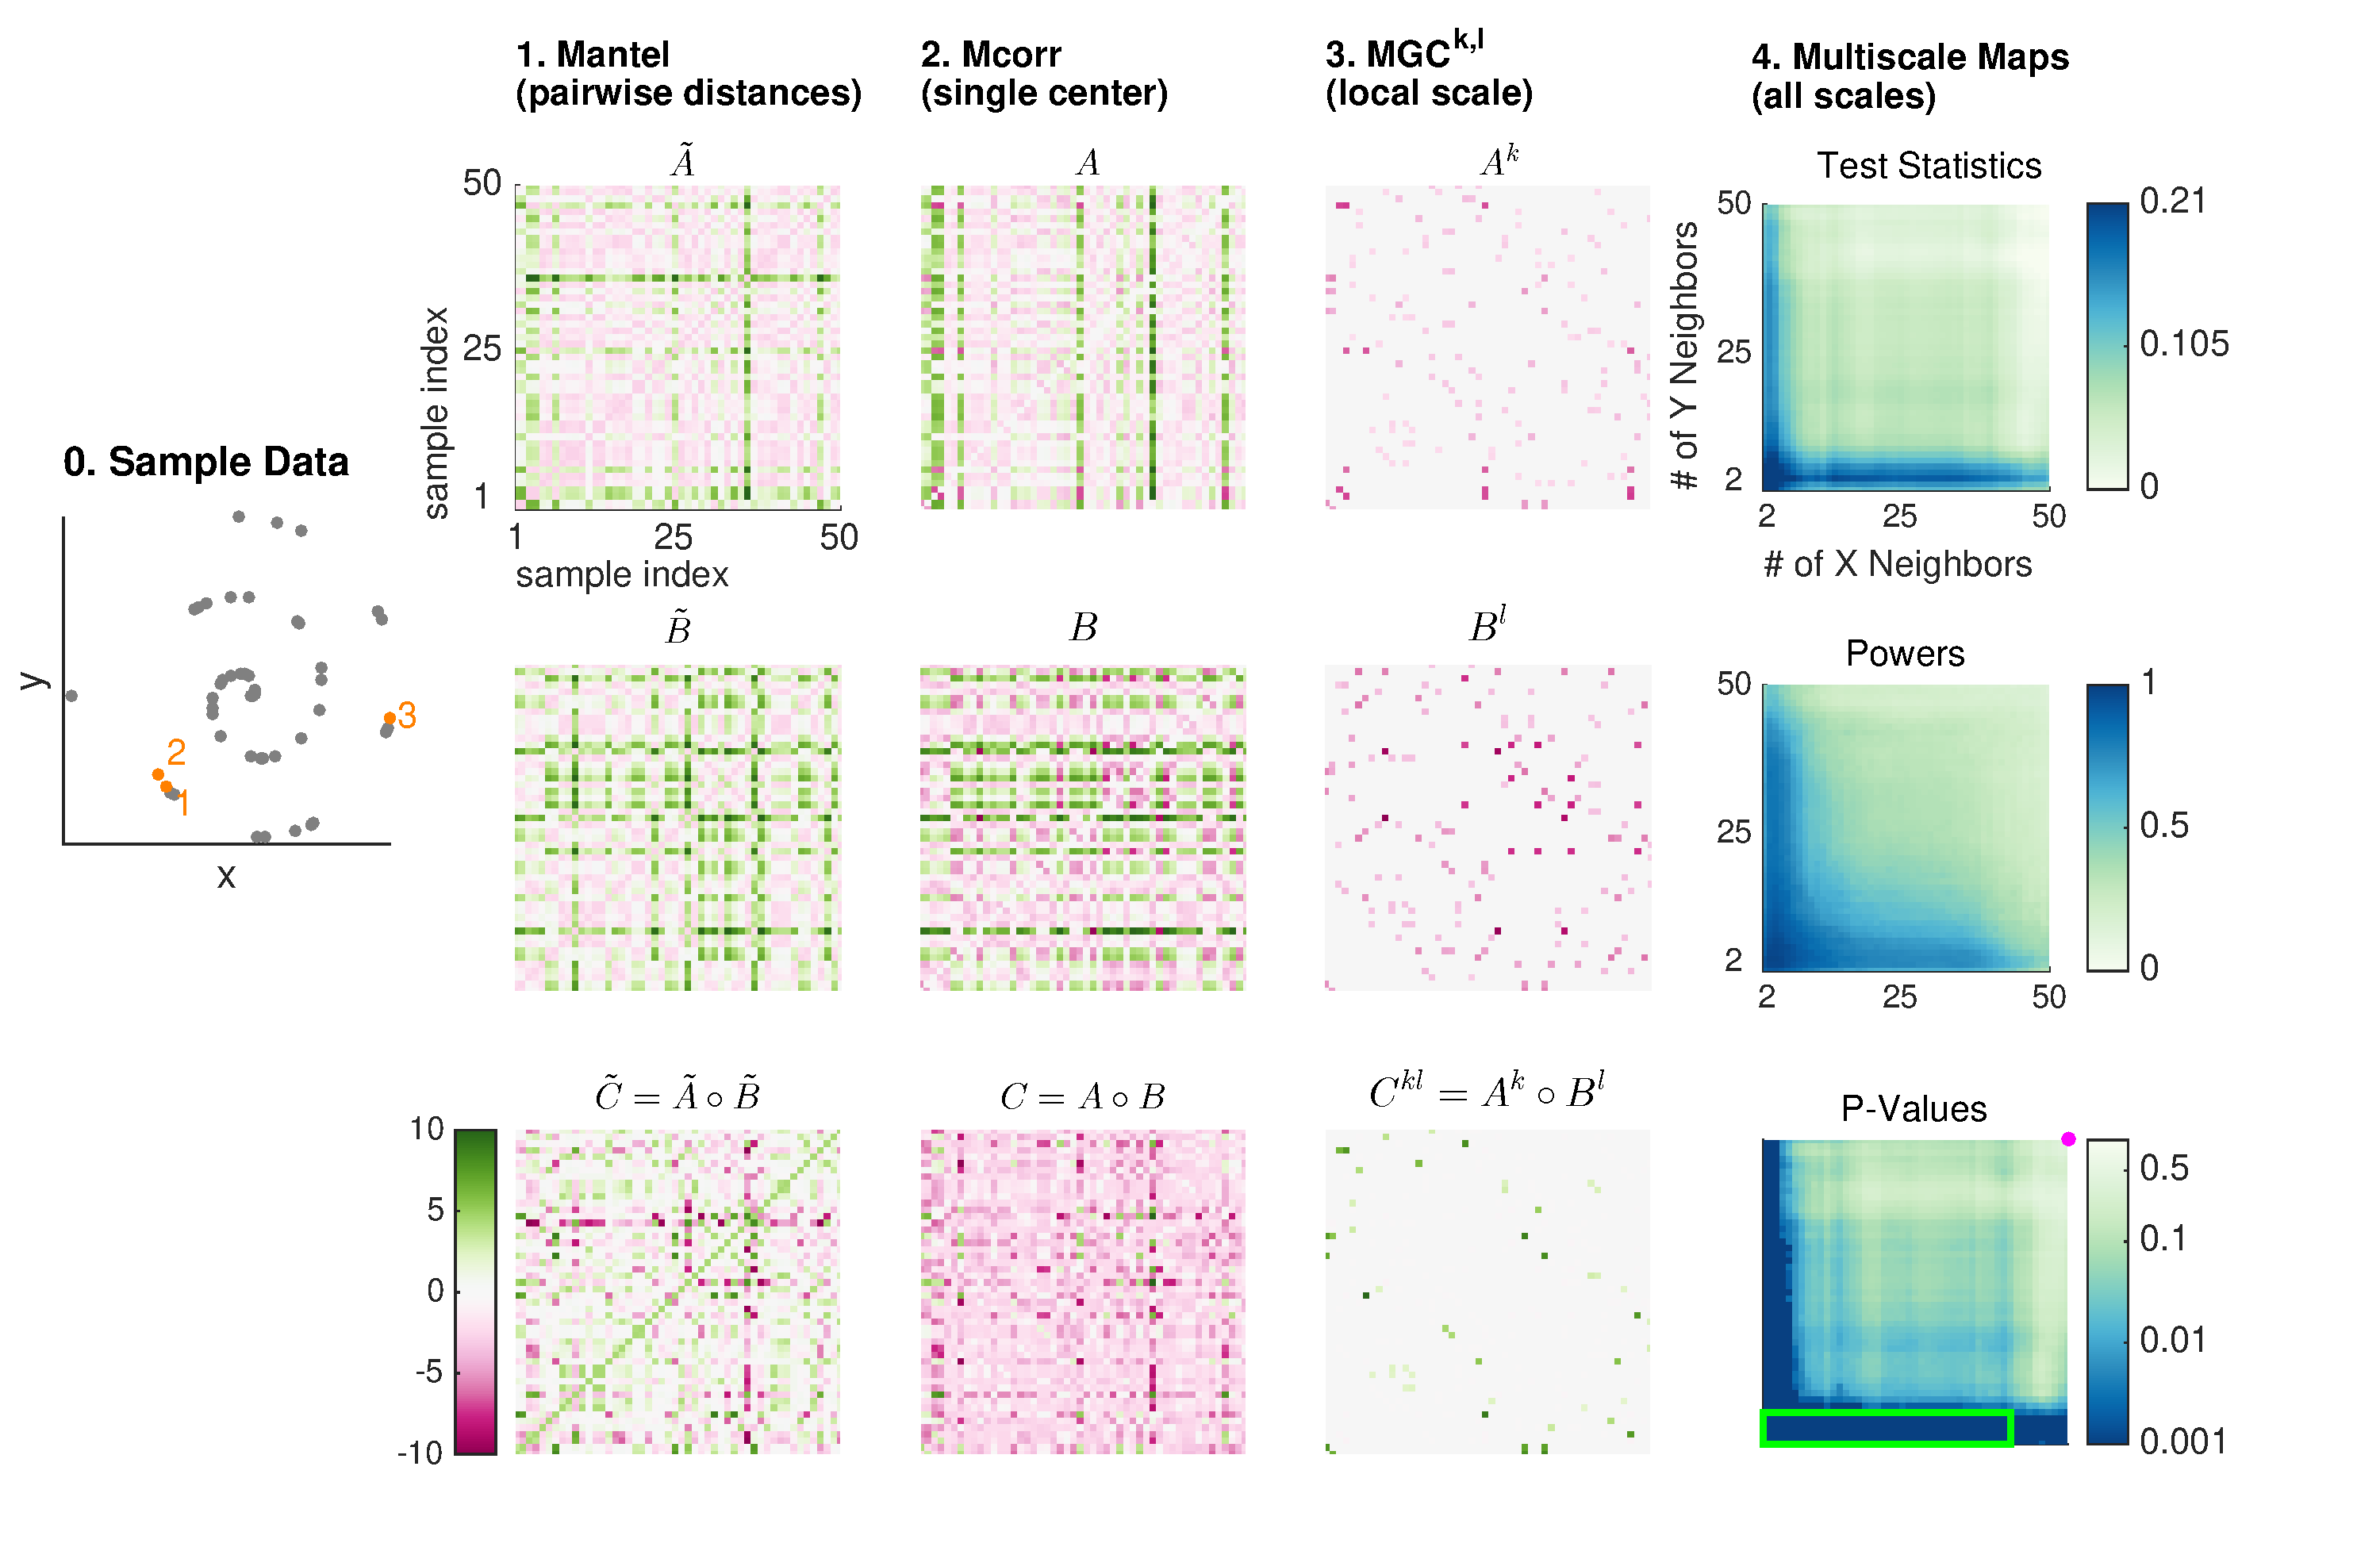
\includegraphics[width=0.9\textwidth,trim={5cm 0 0 0},clip]{../Figures/FigA.pdf}
% \begin{table}
% \caption{ }
% \label{t:mgc}
% \begin{center}
% \vspace{-35pt}\hspace{-150pt}
\setlength{\tabcolsep}{10pt} % Default value: 6pt
% \renewcommand{\arraystretch}{1.5} % Default value: 1
\begin{tabular}{r  r   r   r}
 $\delta_x$(1,2) &  \color{magenta}-2.42  & \hspace{2.8em} \color{magenta}-5.21  &  \hspace{2.6em} \color{magenta}-5.07  \\ 
 $\delta_y$(1,2) & \color{magenta}-1.58 & \color{magenta}-0.91 & \color{magenta}-0.12  \\ 
 $\delta_x \times \delta_y$ & \color{green}3.82 & \color{green}4.74 & \color{green}0.61  \\ 
 
\hline

 $\delta_x$(2,3) & \color{green}0.70 & \color{green}0.61 & \color{green}0.14  \\ 
 $\delta_y$(2,3) &  \color{magenta}-0.91 & \color{magenta}-0.28 & \color{green}0.12  \\ 
 $\delta_x \times \delta_y$ & \color{magenta}-0.63 & \color{magenta}-0.17 & \color{green}0.02  \\ 

\hline
 $\sum{\delta_x \times \delta_y}$ & \color{magenta}-162.14   & \color{magenta}-93.04 & \color{green}116.41  \\ 
 test statistic &  \color{magenta}-0.02  & \color{magenta}-0.02 & \color{green}0.16  \\  
% $\sum{\delta_x \times \delta_y}/z_{xy}$
% $\sum{\delta_x \times \delta_y} / \sum{\delta_{x}^2}\sum{\delta_{y}^2}$ 



\end{tabular}
\jv{the figure and table may need to be re-aligned. }
% \end{center}
% \end{table}
\caption{(caption on next page.)}
\label{f:schematic}
\end{figure}


\addtocounter{figure}{-1}

\begin{figure}[htbp]
\caption{
%\begin{minipage}
Flowchart schematizing Multiscale Generalized Correlation (\Mgc). Columns listed from left to right.
\textbf{Column 1:} 50 pairs of observations $(x_i,y_i)$ are nonlinearly (spirally) dependent on one another.
% 
\textbf{Column 2:} Compute all pairwise distances for $x$ and $y$ yielding interpoint comparison matrices
 $\tilde{A}$ (top) and $\tilde{B}$ (middle), 
and their element-wise product $\tilde{C}$ (bottom), whose normalized sum is the  \Mantel~statistic \cite{Mantel1967}.
Note that implementing it requires choosing appropriate distances for both $x$ and $y$.  
% 
\textbf{Column 3:} Double centering---subtracting the row-sums and column-sums to eliminate bias due to individual samples---yields $A=\{a_{ij}\}$ and $B=\{b_{ij}\}$, which we use to compute $C$, whose normalized sum is the \Mcorr~statistic \cite{SzekelyRizzo2013a}.
% 
\textbf{Column 4:} Rank truncating yields $A^{k}$, $B^{l}$, and $\G^{k,l}$ at $k=l=4$.  $k$ and $l$ can be chosen using either the multiscale p-value or power map, the \Mgc~test statistic is the normalized sum of the elements of $\G^{k,l}$.
All tests detect dependence only when their normalized sum is large.
 % for a particular choice of $(k,l)=(4,6)$ (which is one optimal scale in this simulation), from which we can compute $C^{k,l}$, whose  sum is the \Mgc~statistic.  
\textbf{Column 5:} (Top) The empirical null distribution for \Mcorr, as well as our \Mgc, and the corresponding observed test statistics for each. 
% \Mcorr, the global test, has  p-value $0.067$ while \Mgc, our multiscale test, has  p-value $0.005$.
Multiscale  maps are used to determine the optimal scales, using p-values (middle)  in the absence of the true distribution or training data, and simulated power (bottom) for Oracle \Mgc.  
% Both maps enable one to select the optimal scales and understand the structure of dependence.
Whereas \Mcorr, the global test, has very low power and therefore yields a non-significant p-value ($0.827$),  there are many local scales that achieve nearly perfect power, resulting in highly significant p-values ($\approx 0.005$), as well as revealing the scales of dependency. Table illustrating how \Mgc~is able to detect dependence even in highly nonlinear and low-sample size settings. The three colored points in the scatter plot indicate the three points considered in this table. \Mgc~detects local dependence across $x$ and $y$, whereas the global methods fail to detect significant dependence because certain pairs have large distances in $x$ but not $y$, or vice versa, and global methods fail to discard such pairs.}
 %\end{minipage}}
\end{figure}
\clearpage



\clearpage
Having defined how to compute \Mgc, we face three challenges to make the method practical. First, in addition to the test statistic, we need to compute the null distribution, so that we may find the critical values and p-values.
Second, na\"ively, computing all local $\G^{kl}$ statistics would require an unacceptably large computational budget.
% require $\mc{O}(n^4)$, because it requires $\mc{O}(n^2)$ time to compute each local statistic (Algorithm \ref{alg:1scale} in Appendix \ref{appen:algorithms}).  That computational burden would be so high as to make doing so impractical.
Third, having computed all local statistics, we require a method for choosing the optimal neighborhood sizes, in such a way that the test is still consistent and not biased (so the resultant p-value remains valid).

Computing the p-values from the test statistic is  straightforward.
% , thanks to the advent of permutation testing \cite{GoodPermutationBook}.  
Specifically, we can permute the labels of either the $\mb{x}_i$'s or the $\mb{y}_i$'s, and then compute the \Mgc~statistics on the permuted data \cite{GoodPermutationBook}.  Permuting the labels renders the two different data modalities  independent.  Doing so many times yields an empirical estimate of the null distribution, which we can use to compute the critical value and p-value. This procedure is somewhat time consuming, which makes computing the test statistics for all neighborhoods efficiently even more important.

 % (see Algorithm \ref{alg:all_scales} in Appendix \ref{appen:algorithms} for details on our permutation test).


Nearly all algorithms that employ regularization (for example, sparse methods, feature selection, dimensionality reduction) face a similar dilemma: how to efficiently choose the hyper-parameters.
% requires running the entire algorithm again from scratch.
% Unlike many manifold learning methods,
% once the rank information is given,
% 
Most manifold learning algorithms require that the user essentially runs the entire algorithm again from scratch for each different hyper-parameter setting, a pursuit that can be exponentially taxing as the number of hyper-parameters increases.
In our case, once the rank information is provided, each distance-based local correlation takes $O(n^2)$ time to compute (Algorithm \ref{alg:1scale} in Appendix \ref{appen:algorithms}), which means a na\"ive algorithm to compute all local correlations would take $O(n^4)$ time.
% 
We noted that the sufficient statistics for larger neighborhood sizes include those for the smaller sizes, so we can simply keep track of them as we iteratively increase neighborhood size. 
This insight yields an algorithm for exactly computing \emph{all} local correlations in $\mc{O}(n^2 \log n)$, essentially the same running time complexity as  global correlation coefficients (the additional $\log$ factor is for sorting to find the neighbors  (see Algorithm \ref{alg:all_scales} in Appendix \ref{appen:algorithms} for details). 
The end result is \Mgc~can be computed in  time comparable to the current state-of-the-art dependence tests (see Algorithm \ref{alg:pval} in Appendix \ref{appen:algorithms} for details on computing all $n^2$ p-values efficiently).
% 
% Therefore, we can efficiently compute all local correlations for a given pair of data and the permuted data, which yields the p-values for each neighborhood size (see Algorithm \ref{alg:pval} in Appendix \ref{appen:algorithms} for details). But it does not tell us which neighborhood sizes are optimal.

Finally, we must find the optimal scales. If the underlying joint distribution is known (as in simulations), or can be reasonably estimated via training data, then the optimal scale can be directly estimated by computing power for all local tests and selecting the scale with maximal power, which yields the ``oracle'' \Mgc (see Algorithm \ref{alg:power} in Appendix \ref{appen:algorithms}). In the absence of the true distribution or adequate training data, we cannot reasonably compute power; instead we rely on the p-value map.  Because p-values are noisy, and we are checking many of them, we must guard against overfitting and adding bias.  We do so by searching for consecutive regions of scales for which p-values are consistently low, and approximate \Mgc~p-value within the region (see Algorithm \ref{alg:power} in Appendix \ref{appen:algorithms} for method details). Approximation by p-value map yields the ``sample'' \Mgc, and the sample version is often very close to the oracle \Mgc~as seen in Appendix~\ref{appen:figs} and ~\ref{appen:diss}.
% ). This is the procedure used for real data experiments, which maintains excellent performance 


\subsection*{Finite Sample Simulation Experiments}


We are interested in assessing the performance of our multiscale tests in a wide variety of settings to better understand the tests, and gain insight into which to use in different settings.  
We therefore consider $20$ different joint distributions $f_{xy}$ corresponding to $20$ different noisy dependence settings. A large fraction of these are taken exactly from existing literature \cite{SzekelyRizzoBakirov2007, SimonTibshirani2012, GorfineHellerHeller2012, HellerGorfine2013}, and we have added several additional settings.  They include
linear and nearly linear  (1-5),
polynomial   (6-12),
trigonometric (13-17),
uncorrelated but nonlinearly dependent  (18-19),
and an independent relationship (20).
Details for each setting are given in Appendix \ref{appen:function}, with a visualization of each dependency when $D=D_y=1$ shown in Supplementary Figure~\ref{f:dependencies}. For all $20$ settings, we define  $\delta_x$ and $\delta_y$  as  Euclidean distance, that is, $\delta_x(\mb{x}_i,\mb{x}_j) = \|\mb{x}_i - \mb{x}_j\|_{2}$, and the same for $\delta_y$.


\begin{figure}[htbp]
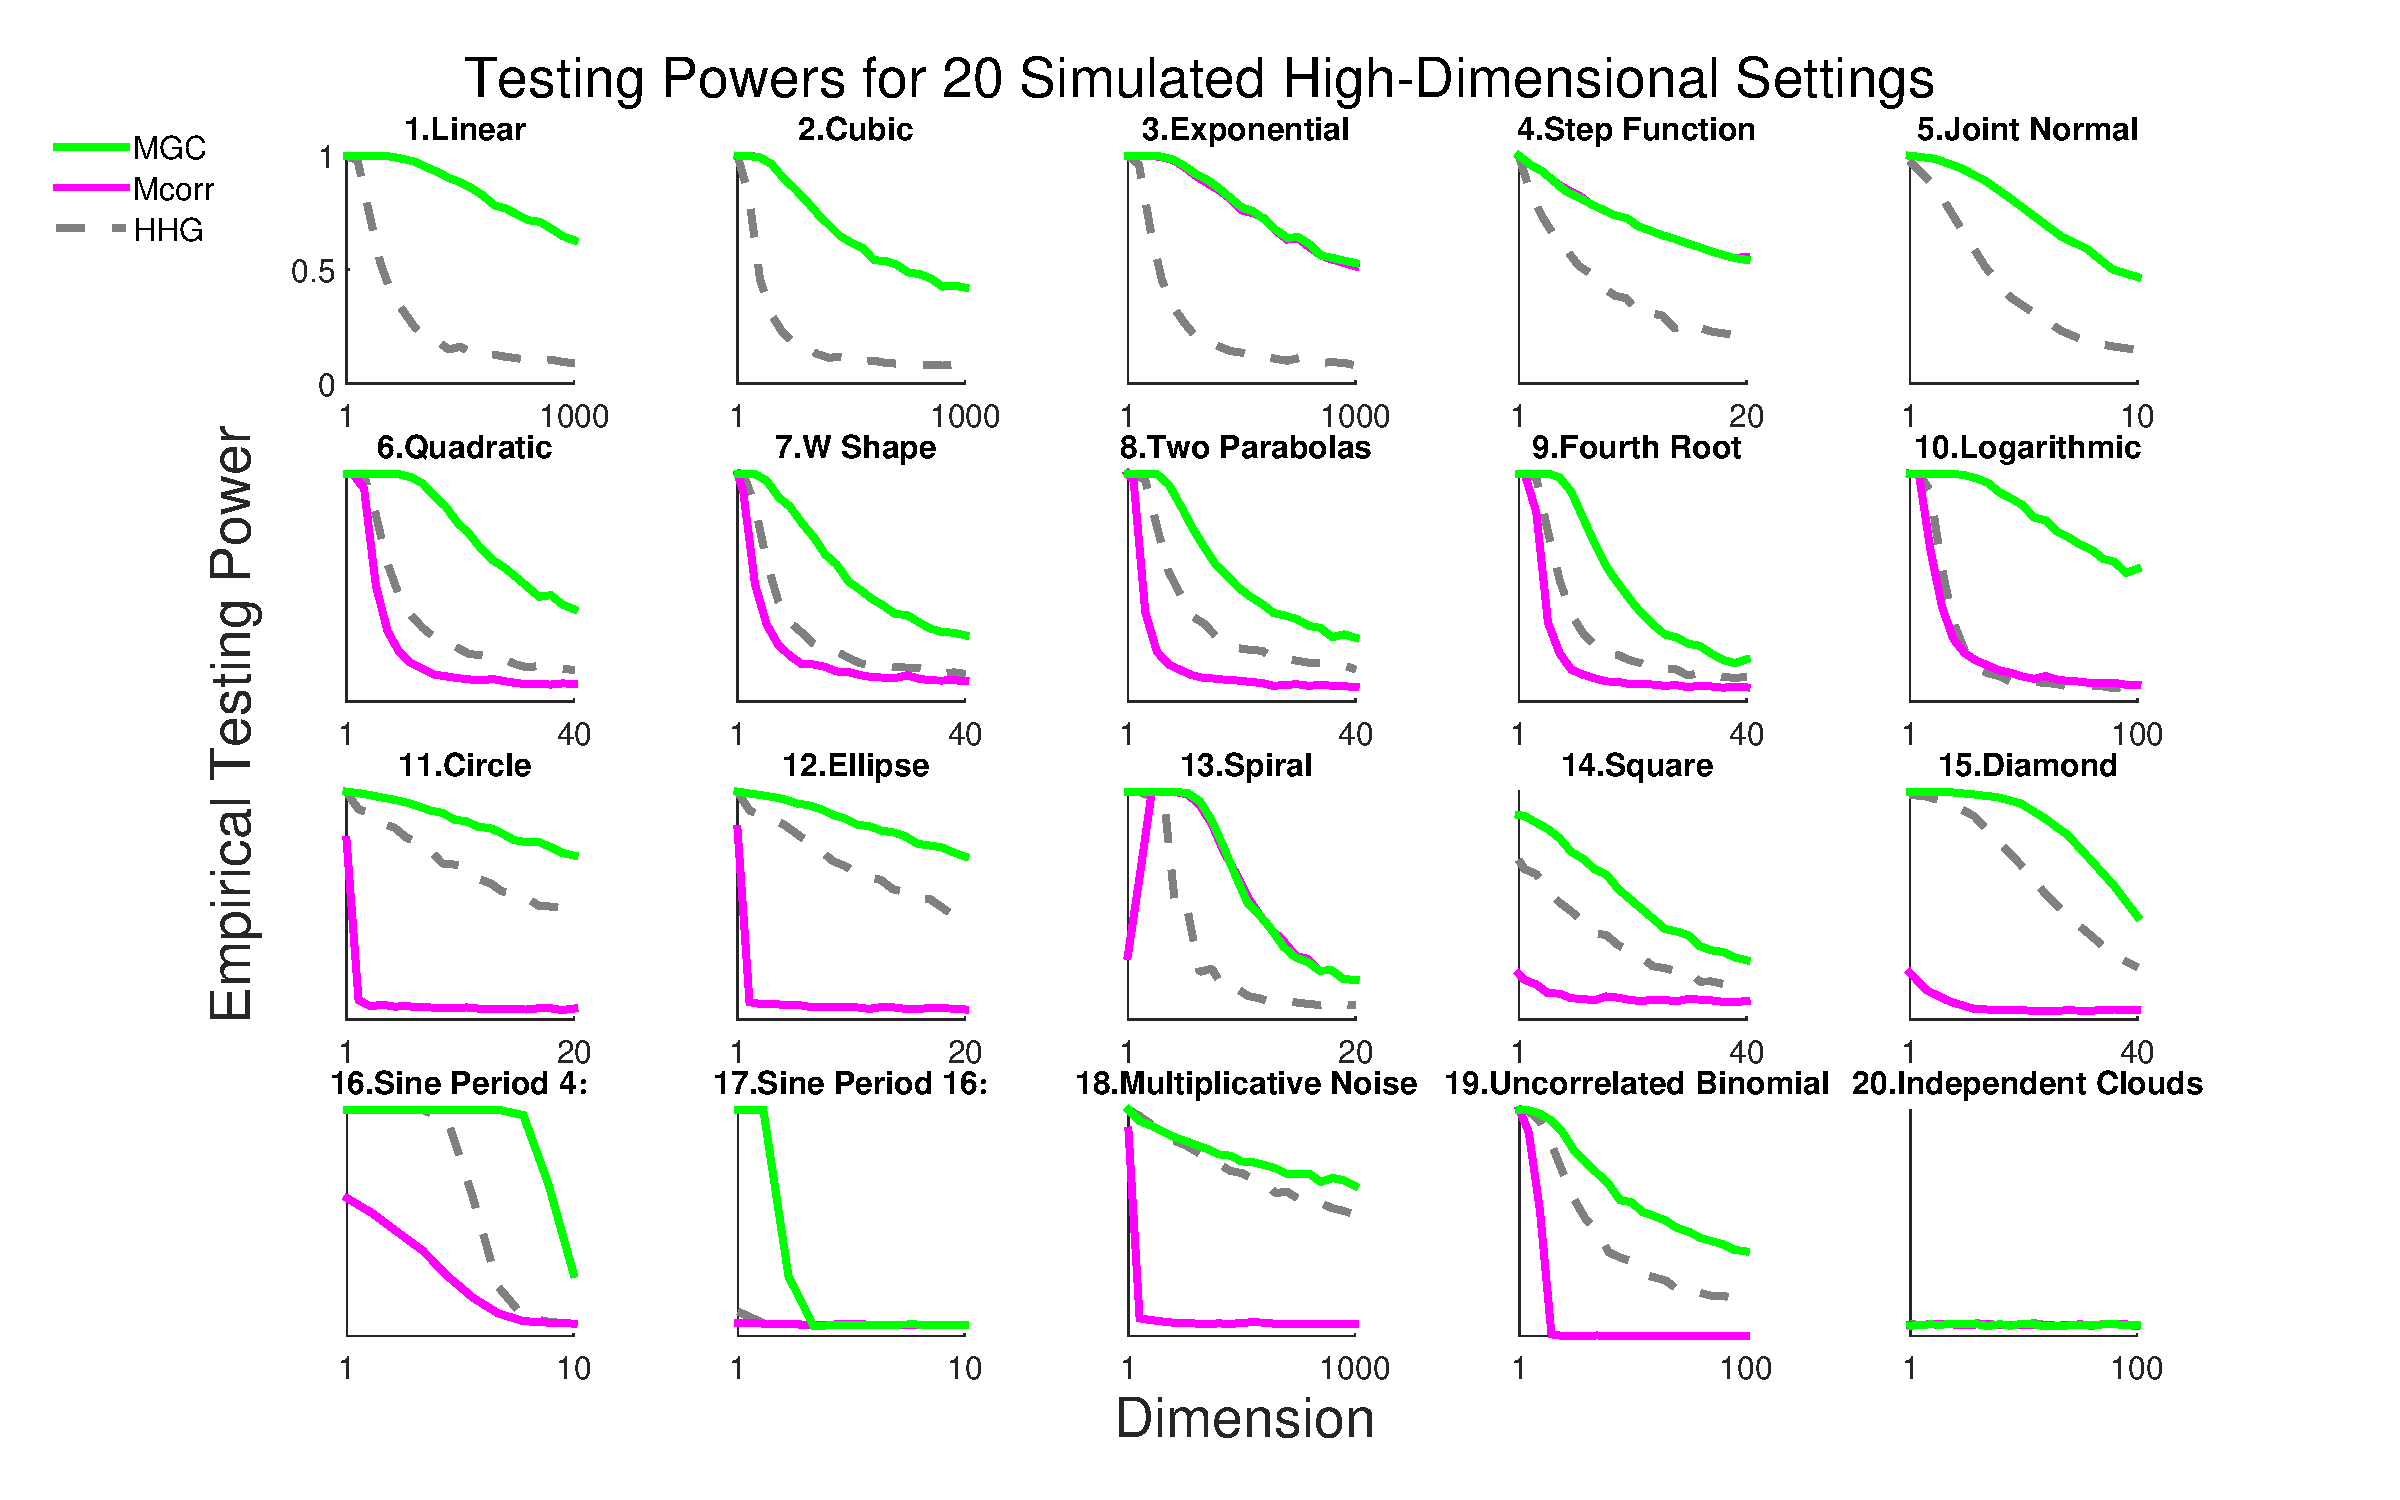
\includegraphics[width=1.0\textwidth]{../Figures/FigHDPower.pdf}
\caption{Powers of \Mcorr, \Hhg, and oracle \Mgc~for $20$ different dependence settings, estimated by Monte Carlo independence tests (see Algorithm \ref{alg:power} in Appendix \ref{appen:algorithms} for details).  
% We used $10$,$000$ Monte-Carlo replicates to estimate the null power, and an additional $2$,$000$  replicates to estimate the optimal scale.
Each panel shows empirical testing power at a significance level $\alpha=0.05$
versus the dimensionality of $\mb{x}$'s, for $n=100$ samples (the dimensionality of $y$ increases for some settings, see Appendix \ref{appen:function} for details). 
Except the independent clouds (setting 20), for which all methods yield power $0.05$, as they should, \Mgc~empirically achieves similar or better power than both \Mcorr~\cite{SzekelyRizzo2013a}, its global counterpart, and \Hhg~\cite{HellerGorfine2013}, another state of the art method, for almost all settings and all dimensions, 
}
\label{f:nD}
\end{figure}



Figure~\ref{f:nD} shows the testing powers versus the dimensionality of \mbx~(the dimensionality of \mby~increases in only a subset of the settings; see Methods for details), with the sample sizes fixed at $n=100$ for each setting.  We compare  our \Mgc with two previously proposed state-of-the-art tests: \Mcorr~\cite{SzekelyRizzo2013a} and \Hhg~\cite{HellerGorfine2013}.  \Hhg~has previously been demonstrated to perform very well on all sorts of nonlinear dependencies, especially in low-dimensional settings, and enjoys strong theoretical guarantees. 
% 
The advantage of oracle \Mgc~over its global counterpart \Mcorr~and \Hhg~is  stark. For the nearly linear settings, \Mgc~and \Mcorr~are essentially identical and significantly better than \Hhg~as the dimension increases.  For the remaining nonlinear dependencies, \Mgc~achieves superior power than \Hhg~and \Mcorr~for almost all functions, often by a significant margin.  For the independent simulation, all tests yield powers at the significance level $\alpha$,  indicating no more false positives than expected according to the theory.
More exhaustive benchmark experiments, including focusing on the one-dimensional scenarios,
in which we also compare to \Mantel~and \Dcorr, 
as well as our  multiscale variants of both \Mantel~and \Dcorr, 
 are qualitatively similar, and are therefore relegated to Figure~\ref{f:1DAll} and~\ref{f:nDAll}.



\subsection*{\Mgc~Empirically Dominates Global Counterparts}

The above results demonstrate that converting \Mcorr, a global generalized correlation coefficient, to oracle \Mgc, its multiscale variant, always improves (or does not diminish) the testing power for all considered settings, regardless of the dimensionality.  We wondered, therefore, whether the multiscale variant of other generalized correlation coefficients would behave similarly.  Specifically we consider the \Mantel~and \Dcorr~tests, in addition to \Mcorr, and for each, develop a multiscale variant (see Appendix \ref{appen:methods} for details). 
% 
Figure \ref{f:pp} show slopegraphs comparing each of the three global correlation and their corresponding oracle \Mgc~test.  The top row shows for each of the $20$ settings, with dimensionality of \mbx's and \mby's  fixed at one, the  power for different sample sizes as in Figure~\ref{f:1DAll}.  The bottom row shows the same, but   dimensionality of \mbx is increasing while the sample size is fixed at $n=100$ as in Figure~\ref{f:nDAll}.  In all $40$ settings, both low and increasing dimensions, and both fixed and increasing sample sizes, multiscale methods always improve on or stay the same, and never decrease power. 
Figure \ref{f:simPerm} shows the distribution of powers for the 20 different simulation settings, for both one-dimensional and high-dimensional cases, comparing power estimated using p-value maps, rather than power maps.  
% using the true \Mgc~power, the \Mgc~power estimated via our p-value neighborhood search, as well as \Mcorr~and \Hhg~for reference. 
Even when estimating the optimal scales via p-values maps, the sample \Mgc~achieves excellent power in nearly all settings, especially high dimensional ones, seee Appendix~\ref{appen:figs}



\begin{figure}
  \centering
  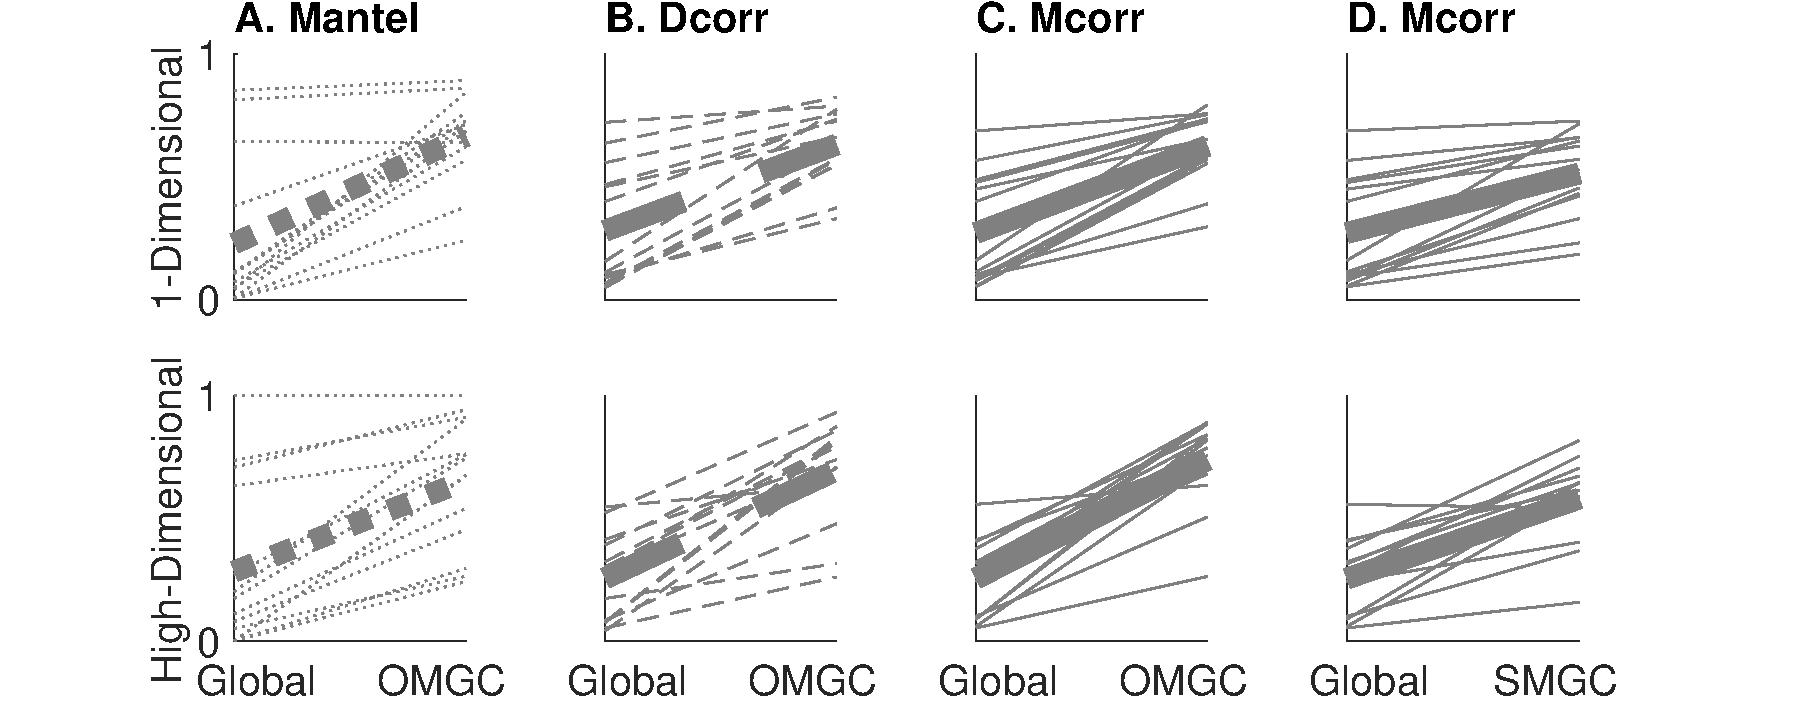
\includegraphics[width=1.0\textwidth]{../Figures/FigSlope.pdf}
  \caption{
Average powers slopegraphs comparing tests by global correlation and the respective oracle \Mgc.  Each panel shows average power for settings 6-19, because \Mgc~equals the global correlation for simulation 1-5 and  20. 
The left side of each panel shows the global correlation's average powers, and 
the right side shows our corresponding \Mgc's average power. The thick line shows the average within that panel. 
One-dimensional power is averaged over sample-size (top)  and increasing-dimensional power is averaged over dimensionality (bottom), corresponding to Figures~\ref{f:1DAll} and ~\ref{f:nDAll}, respectively.
% , and the second row corresponds to high-dimensional simulation powers in Figure~\ref{f:nDAll}. 
This figure suggests that \Mgc~dominates its global counterparts. 
}
\label{f:pp}
\end{figure}

%From Figure~\ref{f:pp}(A)(B), \Mgc~is clearly more reliable than all benchmarks throughout the one-dimensional simulations regardless of the actual implementation. \Hhg~is slightly better than \Dcorr~/ \Mcorr~in the performance profiles, because there are more nonlinear simulations than linear in the $20$ dependencies, and \Hhg~has a larger advantage for nonlinear dependency than its disadvantage in linear dependency; the global \Mantel~test has the lowest performance profile, but utilizing local correlations makes \Mgcp~perform similarly as the other two \Mgc~algorithms.




% 31 lines; target = 64
\subsection*{Discovery of Dependency Across Scales}
\label{main3}

A multiscale power map is a heatmap of powers for all neighborhood sizes, for a given joint distribution and sample size.
Figure~\ref{f:powermaps} provides the multiscale power maps for all 20 different high-dimensional scenarios, illustrating how the powers of local correlations change with  neighborhood size.
% For each panel, the chosen dimension was chosen as the largest one for which $\Mgc$'s power exceeded 0.5, chosen to highlight the differences between scales.
% , for the high-dimensional simulations
%(the one-dimensional case is provided in Figure \ref{f:powermaps1} in Appendix \ref{appen:methods}).
% They are plotted at a fixed sample size and a fixed dimension by the same power thresholds as in Figure~\ref{fig:pp}A and C.
% 
The multiscale power map sheds light into the intrinsic dependency structure.
For nearly linear dependencies (1-5), the best neighborhood choice is always the largest scale, i.e., $k=l=n$. For all strongly nonlinear dependencies (6-19), oracle \Mgc~chooses a smaller scale for $X$ or $Y$.
% in a distribution dependent fashion. 
Furthermore, similar dependencies have similar local correlation structure, and thus similar optimal scales. For example, quadratic (6),  W (7), and two-parabolas are all polynomials of degree 2 with different coefficients, and their power maps are  similar to each other. Similarly,  (16) and (17) are the same trigonometry function (sine) with different periods, and they share a narrow range of significant local correlations.
Both circle (11) and eclipse (12), as well as square (14) and diamond (15), are closely related functions, and have similar multiscale power maps.
% 
Note that for all simulations, there always exists a consecutive region of local scales that are equally significant, which is an important observation that we use to approximate the optimal scales of sample \Mgc~by the p-value map for data of unknown distribution.

\begin{figure}[htbp]
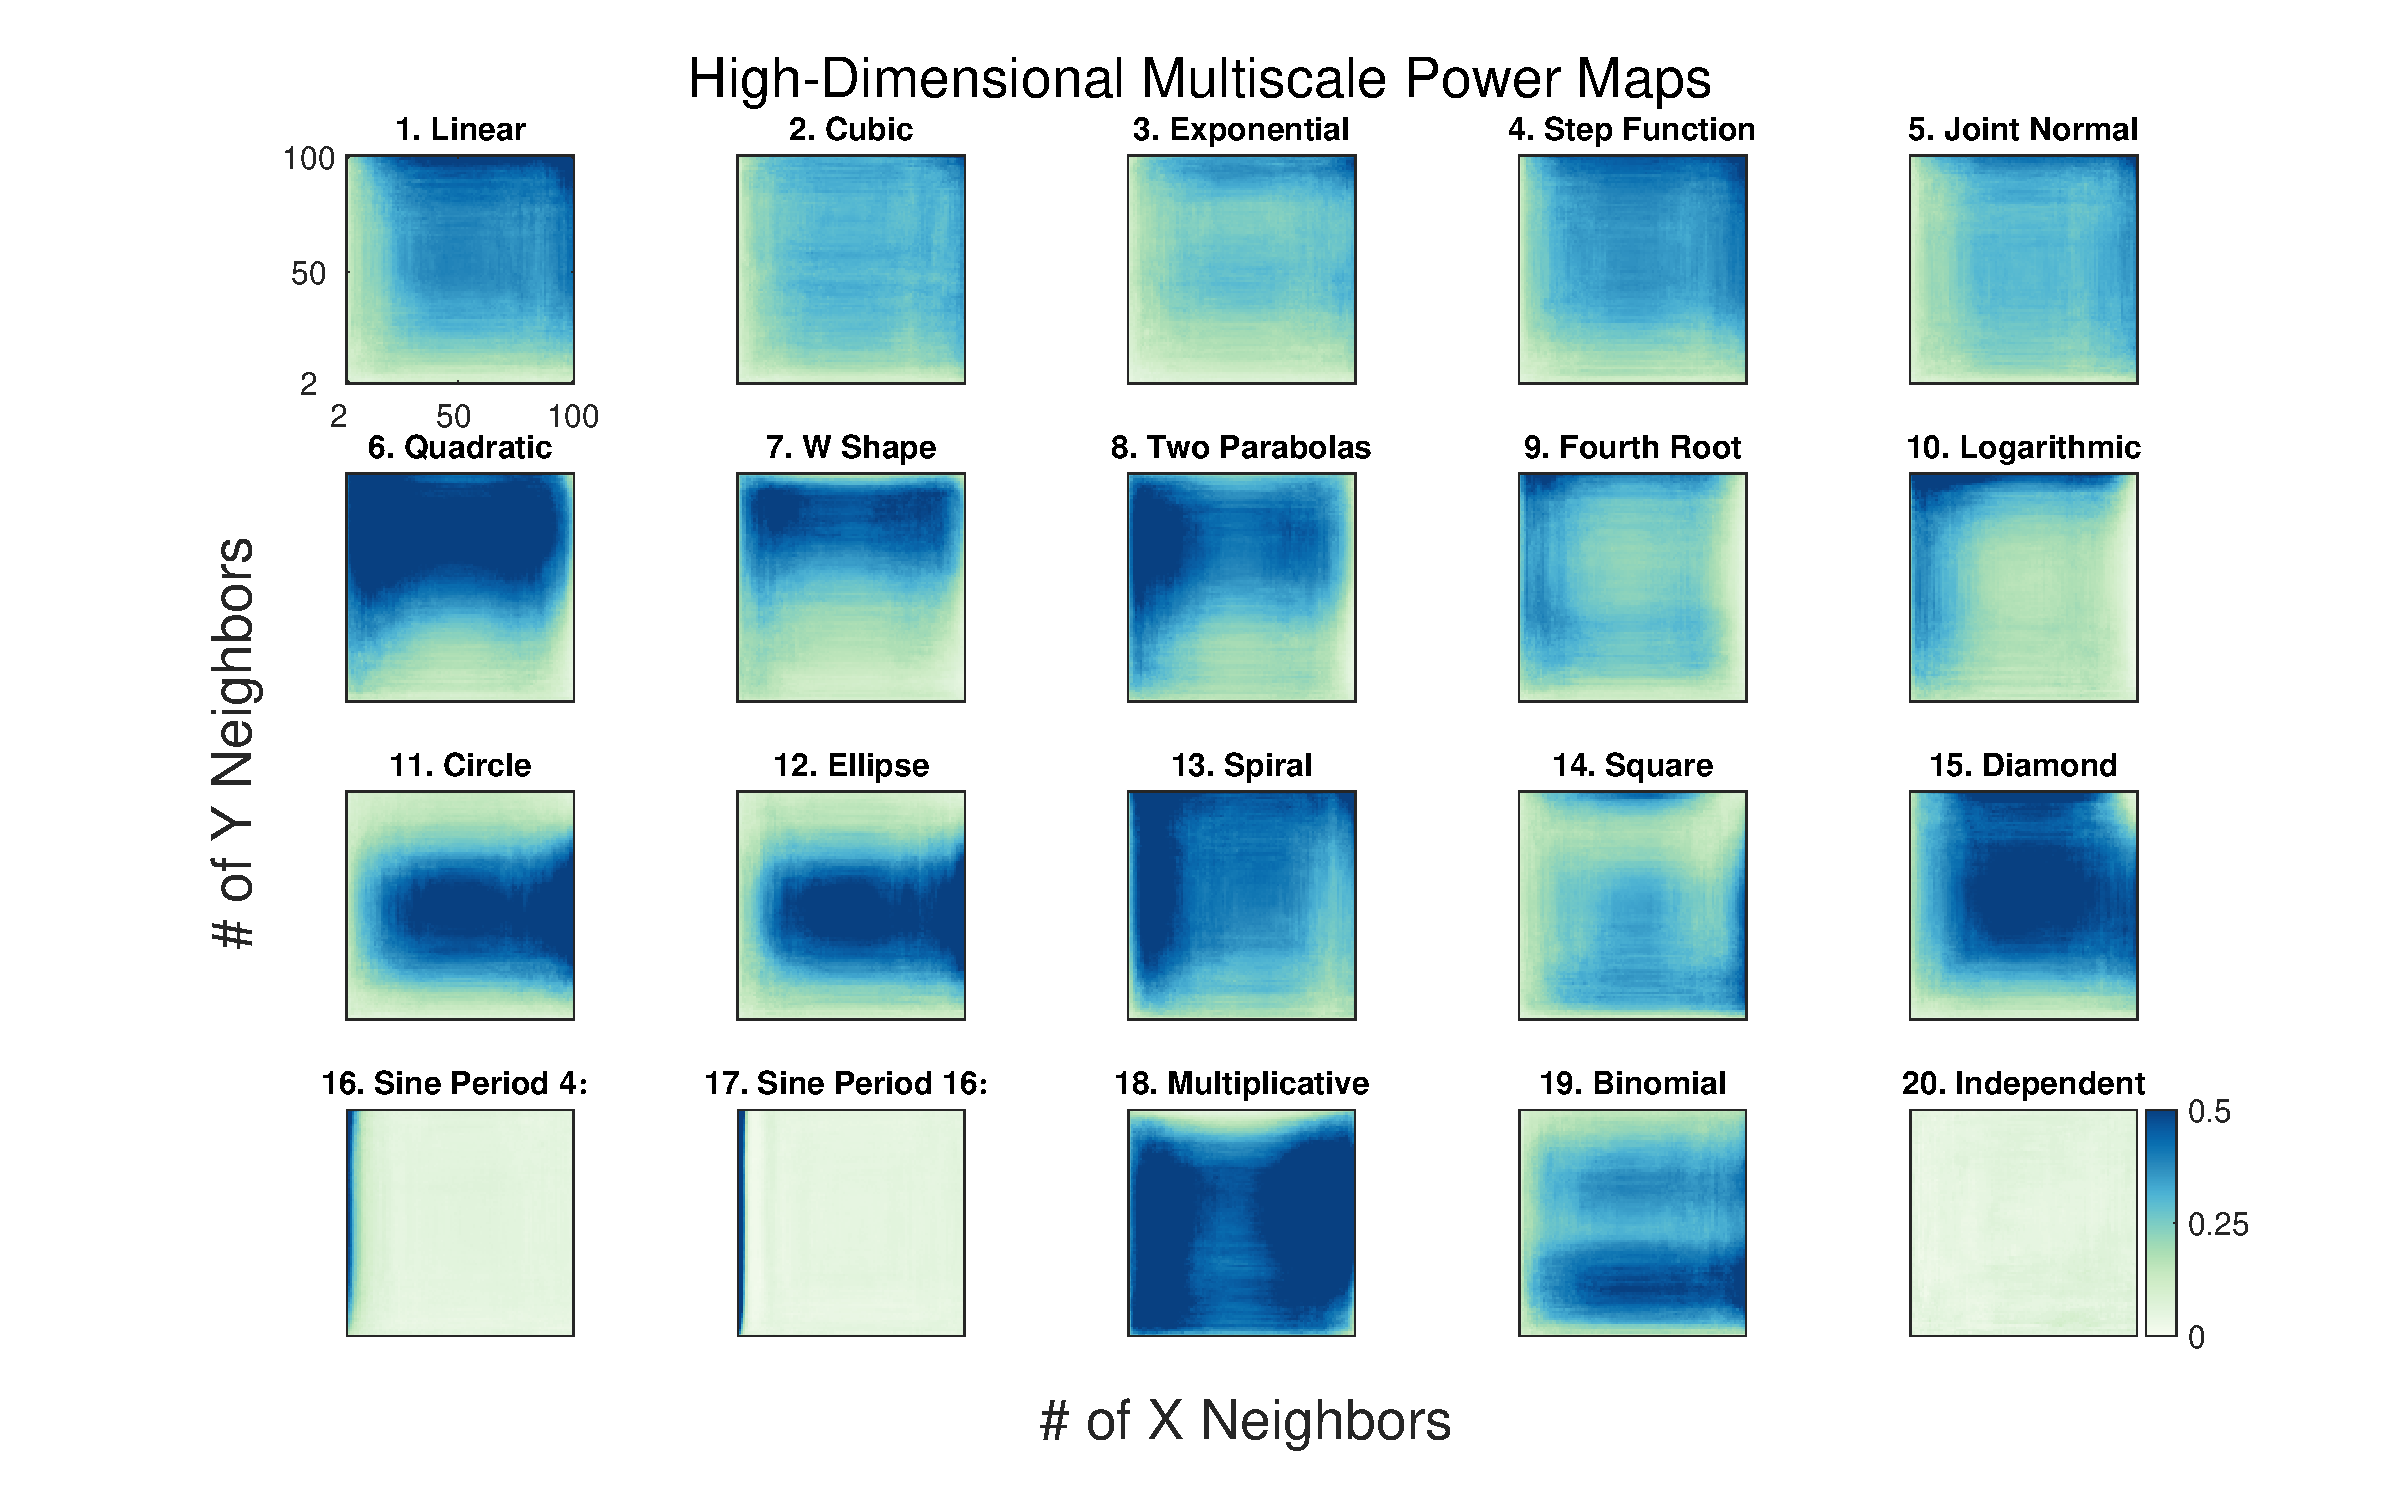
\includegraphics[width=1.0\textwidth]{../Figures/FigHDHeat.pdf}
\caption{Multiscale Power Maps reveal the influence of neighborhood size on \Mgc~testing power.
For each of the 20 panels, the abscissa and orginate denote the number of neighbors for $X$ and  $Y$, respectively. For each simulation, the sample size is $n=100$,  the dimension is determined by the largest dimension for oracle \Mgc~to have power exceeding $0.5$ at significance level  $0.05$. Each simulation yields a different multiscale power map, highlighting that \Mgc~reveals, rather than the mere existence of dependency, also its  structure  (see Appendix~\ref{appen:mgc} for details).}
\label{f:powermaps}
\end{figure}


\subsection*{\Mgc~Theoretically Dominates its Global Counterparts}
\label{s:theory}

The formal testing scenario is as follows: we observe $n$ pairs of observations, $\{(\mb{x}_i,\mb{y}_i)\}$, and we desire to know whether the \mbx's are independent of the \mby's.  To cast this problem as a statistical inference query requires specifying a statistical model, that is, a collection of possible distributions from which we may assume the data arise.  To make the investigation as general as possible, we consider the largest possible set of distributions: any possible joint distribution $f_{xy}$. If \mbx~and \mby~were independent, then it would follow that $f_{xy}=f_x f_y$; in other words, for independent data, the joint distribution is equal to the product of the marginals.  Therefore, we have the following hypothesis testing scenario:
\begin{align*}
& H_{0}: f_{xy}=f_{x}f_{y},\\
& H_{A}: f_{xy} \neq f_{x}f_{y}.
\end{align*}
% where $f_{xy}$ denotes the joint distribution of $(\mb{x},\mb{y})$.

The power of a test is defined as the probability that it correctly rejects the null when the null is indeed false, and has power equal to the type $1$ error level when the null is true.
As defined above, a test is consistent if its power converges to unity as sample size increases when $f_{xy} \neq f_x f_y$.
Let $\G_t$ denote a global generalized correlation coefficient based test statistic, that is, $t$ might indicate \Mantel, \Dcorr, or \Mcorr, and let $\beta(\G_t^*)$ denote the power of the corresponding multiscale version.
Recall from the work Szekeley et al. that \Dcorr~and \Mcorr~are both consistent tests. More specifically, \Dcorr~is consistent whenever $f_{xy}$ has finite dimension and bounded variance, and \Mcorr~is consistent even as dimension increases to infinity.  Denote the set of distributions satisfying consistency for a given test by $\mc{F}_t$, where $t$ indicates which test we are referring to. Then, we have the following theorem:
 % in different scenarios, leads us to our first theorem.
% A consistent test statistic has power $1$ asymptotically, i.e., the test statistic under the alternative is asymptotically larger than the statistic under the null. Denote the type 1 error level as $\alpha$, the testing power of \Mgc~as $\beta_{\alpha}(\G^{*})$, and the power of the respective global test as $\beta_{\alpha}(\G)$. Assuming the optimal scale is estimated by the testing power, we have the following theorem regarding the consistency of \Mgc, whose proof is provided in Appendix \ref{appen:proofs}:
\begin{thm}
\label{thm1}
$\beta(\G_t^*) \rightarrow 1$ for all $f_{xy}$ in $\mc{F}_t$.
In words, oracle \Mgc~is consistent against all dependent alternatives for which its global counterpart is. 
% whenever $\beta(\G)$ does.
% Suppose for given $f_{xy}$ and $\alpha$, $\beta_{\alpha}(\G) \rightarrow 1$ as $n \rightarrow \infty$, then $\beta_{\alpha}(\G^{*}) \rightarrow 1$ as well.
\end{thm}

% 
% Asymptotic consistency, however, does not convey to us how quickly \Mgc~achieves optimal power in various settings, and whether it exhibits significant advantage over its global counterpart and other popular methods.  For that, we turn to numerical simulations.
For finite samples, we consider two different kinds of dependencies.
% The above described qualitative descriptions led us to believe the following two conjectures.  
For linear dependencies,  the optimal \Mgc~scale was empirically always the global one (recall Figures~\ref{f:1DAll} and \ref{f:nDAll}). We therefore conjectured and proved the following:
\begin{thm}
\label{t:linear}
If $\mb{x}$ is linearly dependent on $\mb{y}$, then for any $n$ it always holds that
\begin{equation}
\beta(\G^{*}_t) = \beta(\G_t).
\end{equation}
In words, the optimal scale for oracle \Mgc~is the global scale for linearly dependent data.
\end{thm}

Under nonlinear dependencies and finite sample sizes (which better characterizes essentially all real data), we noted that \Mgc~typically achieved better power than its corresponding global correlation. 
% On the other hand, for finite sample nonlinear dependencies (which better characterize all real data), we note that \Mgc~almost always \emph{improves} upon its global counterpart.  
We therefore conjectured and proved the following:
\begin{thm}
\label{t:non}
There exists $f_{xy}$ and $n$ such that
\begin{equation}
\beta(\G^{*}_{t}) > \beta(\G_{t}).
\end{equation}
In words, for finite samples, \Mgc~can be better than its global correlation coefficient under certain nonlinear dependency.
\end{thm}
Note that Theorem~\ref{t:linear} and Theorem~\ref{t:non} hold for any of \Mgc~varieties, including  \Dcorr, \Mcorr, and \Mantel.
%
The proofs of Theorem~\ref{t:linear} and \ref{t:non} are both in Appendix \ref{appen:proofs}.  The proof of Theorem~\ref{t:linear} is straightforward.  The proof of Theorem~\ref{t:non} is a constructive one. More specifically, we constructed a quadratic function and sampled data a finite number of times and exactly compute the p-value for both \Mgc~and \Dcorr, proving that \Mgc~has higher power in this setting. This shows that \Mgc~can outperform its global counterpart even for the most modestly nonlinear functions.  Because any function can be approximated by a polynomial expansion \cite{RudinBook}, the proof of Theorem~\ref{t:non} suggests that \Mgc~is able to outperform its corresponding global correlation on a wide variety of nonlinear functions, which is indeed the case throughout the numerical simulations. %To our knowledge, Theorems \ref{t:linear} and \ref{t:non} are the first finite sample theorems for dependence testing.

The three above theorems taken together lead to the main theoretical result of this manuscript:
\begin{thm}
Oracle \Mgc~dominates its global counterpart, meaning that \Mgc~is always as good as, and sometimes better than, its corresponding global correlation coefficient, even in finite samples. 
\end{thm}

To our knowledge, this is the first domination theorem in dependence testing.


\subsection*{Real Data Experiments}
\label{numer3}

\subsubsection*{Brain activity and personality} % Between Hippocampus Shape and Depression}
Our first real data experiment investigates whether there is any dependency between the brain activity and personality.
% , from a data set of small sample size and high-dimensionality. 
Adelstein et al. \cite{AdelsteinEtAl2011} was able to detect dependence between certain regions and dimensions of personality, but lacked the tools to test for dependence of the whole brain activity against all five dimensions of personality. 
% If dependence is weak for individual edges or dimensions of personality, then dependence might only be discovered upon considering the joint statistics.
% There exists certain relationship between the brain activity and personality as shown in \cite{AdelsteinEtAl2011}, but existing statistical tests fail to discover any significant dependency from the raw data.
In this dataset, we have $n=42$ subjects, for each we obtained  $197$ time-steps of resting-state functional MRI activity, as well as her five-factor personality trait as quantified by  the NEO Personality Inventory-Revised  \cite{Costa1992}. 
% The data set contains $n=42$ subjects, where each person's personality is assessed by a questionnaire utilizing the five-factor personality model. 
The raw brain activity was processed using CPAC \cite{CPAC2015} resulting in $197$ brain regions.
 % for $194$ time steps. 
% Thus the brain connectome modality is high-dimensional while the personality data is low-dimensional. 
To apply \Mgc, two metrics are required. For the brain activity modality, we ran a spectral analysis on each region, bandpassed and normalized it, and then calculated the Kullback-Leibler divergence across regions and the normalized Hellinger distance between each subject. 
For the five-factor personality data, we  use the Euclidean distance.


% and personalities are independent of one another. Previous work \cite{AdelsteinEtAl2011} investigated whether individual voxels were related to specific dimensions of personality, but were unable to compare entire brain networks to a higher-dimensional characterization of personality. 


% Figure \ref{f:real}A provides the p-value map of \Mgc
% , based on $r=10$,$000$ random permutations. 
Figure \ref{f:real}A  shows that many local scales yield significant p-values (around $0.01$), whereas the global scale fails to detect this significant dependence. The previously proposed dependence test under consideration (\Mantel, \Dcorr, \Mcorr, or \Hhg) also all fail to detect dependence at a significance level of $0.05$. The sample \Mgc~p-value is $0.0343$ by Algorithm~\ref{alg:best_scale}, followed by \Hhg~at $0.0588$, with all others have p-values higher than $0.3$.


\subsubsection*{Brain shape and disease} % Between Hippocampus Shape and Depression}


Our next experiment investigates whether brain shape and disease status are dependent on one another.  Previous investigations have linked major depressive disorder to the hippocampus shape \cite{ParkEtAl2008,PosenerEtAl2003}, though global tests were unable to detect a statistically significant dependence structure at the $\alpha=0.05$ level.



This brain shape versus disease dataset consists of $n=114$ subjects, for each we have a structural MRI scan as well as a discrete variable indicating whether the subject is clinically depressed $(2)$, high-risk $(1)$, or non-affected $(0)$.  From the MRI data, previous work  extracted both the left and right hippocampi.   For the brain shape modality, they computed the interpoint comparison matrices using a nonlinear landmark matching approach \cite{ParkEtAl2008,BegEtAl2005}. For the discrete disorder variable, we add white noise bounded by $0.01$ to each label, then form the Euclidean distance (the noise is used to break ties and make sure only the diagonal entries of the distance matrix are zero).

We consider two dependence tests, one for each hemisphere: is hippocampus shape independent of depressive state.
% testing dependency between the left brain and major depressive disorder, and testing dependency between the right brain and major depressive disorder.
% The resulting p-values based on $r=10$,$000$ random permutations are reported in the first two rows of Table~\ref{table1}. For testing between the left brain and the disorder, \Mgc~/ \Hhg~/ \Mantel~yield significant p-values with \Dcorr~/ \Mcorr~being slightly higher than significance; for testing between the right brain and the disorder, only \Mgc~yields significant p-value, and all benchmarks have p-values higher than significance.
Figure \ref{f:real}B provides the p-value map for testing on right hemisphere using \Mgc. Again, many local scales yield significant p-values, whereas the global scale does not detect a significant dependence. The approximate sample \Mgc~p-value is $0.0205$, and no other dependence tests can identify the underlying  dependence. The left hemisphere seems less dependent on disease status, 
% is more globally dependent on disease: 
% however, \Mgc~equals the corresponding global correlation, and 
both local and global tests yield  p-values from $0.05$ to $0.08$ (not shown). 
\jv{let's check whether anybody knew that?}

% \begin{table*}[!t]
% \caption{The p-values by the permutation test, for testing dependence on $4$ different pairs of real data. Significant p-values are highlighted. \Mgc~is able to consistently identify significant relationship for the first three rows, and does not inflate the p-value in the last row.
% % \Large
% \renewcommand{\arraystretch}{0.5}
% \centering
% {\begin{tabular}{|c||c|c|c|c|c|c|c|}
% \hline
% Testing Method & \Mgc~& \Dcorr~& \Mcorr~& \Mantel~& \Hhg~\\
% \hline
% Left Brain vs Disorder  & $\textbf{0.0046}$ & $0.0745$ & $0.0783$ & $\textbf{0.0382}$ & $\textbf{0.0375}$ \\
% \hline
% Right Brain vs Disorder & $\textbf{0.0133}$ & $0.1046$ & $0.1104$  & $0.0848$ & $0.0809$\\
% \hline
% \Migraine~vs CCI & $\textbf{0.0111}$ & $\textbf{0.0088}$ & $\textbf{0.0111}$  & $\textbf{0.0093}$ & $\textbf{0.0341}$\\
% \hline
% % \mtg~vs CCI & $0.0712$ & $0.0682$ & $0.0712$  & $0.3314$ & $0.6553$\\
% % \hline
% \end{tabular}
% \label{table1}
% }
% \end{table*}

\begin{figure}
  \centering
  \begin{tabular}{@{}p{0.24\linewidth}@{\quad}p{0.24\linewidth}@{\quad}p{0.24\linewidth}@{\quad}p{0.24\linewidth}@{}}
	\centering
	\subfigimg[width=\linewidth]{A}{../Figures/FigReal1} &
    \subfigimg[width=\linewidth]{B}{../Figures/FigReal2} &
    \subfigimg[width=\linewidth]{C}{../Figures/FigReal3} &
    \subfigimg[width=\linewidth]{D}{../Figures/FigRealCORR}
  \end{tabular}
\caption{
(A) P-value map of all local correlations for brain fMRI scan vs five-factor personality model.
(B) P-value map for brain right hemisphere vs disease.
(C) P-value map of all local correlations from $k=2,\ldots,109$ and $l=2,\ldots,38$ for brain \Migraine~vs CCI. $l=38$ is the largest possible neighborhood size for the CCI data due to repeated entries.
(D) Density estimate for the false positive rates of sample \Mgc~on the brain vs noise experiments, with the actual rate of each data shown as dots above the x-axis. The mean, median, and standard deviation are $0.0576, 0.0450, 0.0452$ respectively.}
\label{f:real}
\end{figure}

\subsubsection*{Brain structural networks and disease}
% : Brain Structural Network vs. Personality}

The next real data experiment investigates whether brain structural networks are independent of creativity.  Neural correlates of creativity have previously been investigated, though largely using structural MRI and cortical thickness \cite{Jung2009}.  Here, we used data from a previously published result on graph similarity \cite{Koutra15a}. For  $n=109$ subjects, we have both diffusion weighted (DW-) MRI data as well as the subject's ``creativity composite index'' (CCI).  We processed the raw DW-MRI data via \Migraine, a pipeline for estimating brain networks from diffusion data \cite{Migraine}.   
The brain network metric we used was based on  the semi-parameteric test statistic \cite{Tang2016} that tests whether pairs of graphs with labeled vertices are sampled from the same distributino.  This test statistic was developed to reduce  the very high-dimensionality of adjacency matrices via employing adjacency spectral graph embedding  \cite{Sussman2013}. For these data, we chose to embed each graph into two dimensions for simplicity. We use Euclidean distance to compare CCI values. 
\jv{missing migrain citation?}


Figure \ref{f:real}C shows that the global dependence tests can ascertain whether the whole brain-network is independent of the subject's creativity.  However, the global test is quite fragile, even ignoring a single subject from the global test can render the test non-significant. On the other hand, \Mgc~is much more robust: there is a whole region of neighborhood sizes such that the test is quite significant.  

% Moreover, that the local tests performs optimally with approximately 30 neighbors suggests that these data have multiple cohorts, for which the dependence structure likely differs.  


A primary goal of statistical analysis and modeling is to suggest the next experiment or analysis.  For all three of the above investigations, \Mgc~not only found dependence, but also indicated the nature of that dependence.  Specifically \Mgc~provided the scales for which the dependence is strongest.  Thus, to further investigate these datasets---for example, to build a brain-based assay for any of these mental properties---we would start by breaking the data into multiple cohorts, whose sizes correspond to the optimal scales detected here.  Without \Mgc, there would be no dependence test based justification for any subsequent step.

% For all three of the above results, This result therefore suggests  the next investigatory steps to take to further understand the nature of the dependence structure between brain networks and creativity.

% Next we experiment on \Migraine~vs CCI and \mtg~vs CCI. More specifically, we estimated brain graphs from diffusion MRI data using two different pipelines, one called \Migraine, and the other called \mtg.  The question we have is whether brain graphs are independent of personality.  Because we cannot directly measure brain graphs, we must estimate them from the data.  Currently, the jury is out on which estimation procedure is best.  Therefore, we tried two different brain-graph estimation pipelines to determine which worked better for this particular task.

% Using the same testing procedure as the previous experiment, the resulting p-values for \Migraine~vs CCI and \mtg~vs CCI are reported in the last two rows of Table~\ref{table1}. The dependency between \Migraine~and CCI is strong enough for all dependence tests to return significant p-values; in particular, we observe that there exists many local scales with significant p-values for \Migraine~vs CCI from the p-value heat map in Figure~\ref{f:real}(B). But there appears to be a loss of dependency between \mtg~and CCI, as most significant scales for \Migraine are no longer significant when testing on \mtg. (The p-value heat map for \mtg vs CCI is not shown, as it has no significant scale.)

% All the benchmarks also suggest the disappearance of significant dependency, but they do not exhibit the local structure difference. And \Mantel~and \Hhg~are less informative due to the large change of p-values when moving from \Migraine~to \mtg. Note that if we test independence between \Migraine~vs \mtg, the p-values of all tests are $0$, indicating a strong dependency.

% Therefore in this exploration task, \Migraine~is a better brain graph estimator than \mtg: although they are strongly related with each other, \Migraine~is more dependent with CCI than \mtg, because \mtg~is a transformation of \Migraine~without consideration of CCI. Our method identifies the better representation of the two, reveals the local dependency loss from the p-value heat maps, and does not identify false signals. Thus \Mgc~can be used to find the most relevant representation / variable and provide valuable insights into the structural difference.

\subsubsection*{Sample \Mgc~Does Not Inflate False Positive Rates} %: Brain Activity vs. Noise}

In the last experiment, sample \Mgc~is applied to test independence between brain voxel activities and non-existent stimulus similar to a pair of studies led by Eklund et al. \cite{EklundKnutsson2012,Eklund2015}. We considered $25$ resting state fMRI data sets from the 1000 functional connectomes project (\url{http://fcon_1000.projects.nitrc.org/}), consisting of a total of $1583$ subjects.
We used CPAC to estimate regional time-series, in particular, using the sequence of pre-processing decisions determined to optimize discriminability \cite{Wang2016}.  The output for each scan is the resting state fMRI time-series data containing $200$ regions of interest for $200$ time-steps.
We then also generate an independent stimulus  by sampling from a standard normal at each time step.  Of course, the brain activity data and the stimuli are independent by construction.
For each brain region, we test: is activity of that  brain region independent of the time-varying stimuli. We pool brain activity over all of the samples from the population.
Any regions that are detected significant are false positives by definition.  By testing reach brain region separately, we obtain a distribution of false positive rates.  If our test is unbiased, that distribution should be centered around the significance level, which we set at $0.05$ for this experiment.

To conduct this test, we must construct a distance matrix for brain region activity, and another for the stimulus. For each brain region $g$, we compute the Euclidean distance pairs of time steps,  $a_{ij}^g=\|\mb{x}_{\cdot i}^g-\mb{x}_{\cdot j}^g\|_2$,  where $\mb{x}_{\cdot i}^g$ denotes the observation vector of activity of region $g$ at time-step $i$ for all subjects.
For the one-dimensional stimulus, we similarly compute the Euclidean distance between the stimulus values at each pair of time-steps: $b_{ij}= \|y_i - y_j\|_2$.
Note that the distance matrices at different brain regions are distinct, but the stimulus is the same for all brain regions during the same experiment.
% From the two distance matrices, we test the dependency between each brain region and the time-varying stimulus by \Mgc.
% The p-values are based on $1000$ random permutations.

For each data set, the above test is carried out for each brain region; the false positive rates of sample \Mgc~for each dataset are shown in Figure~\ref{f:real}D. %The y-axis stands for FPR by log scale, and the x-axis shows the name of the data set arranged by increasing FPR; the mean FPR of \Mgc~is shown as the purple-red straight line, with the type $1$ error level $0.05$ drawn as the blue straight line.
% Because the stimulus is in fact independent of the brain activities, the false positive rate should be close to $\alpha=0.05$ for each data set.
Sample \Mgc~false positive rate is centered around the critical level $0.05$, as it should be.
% ; the mean/standard deviation is $0.060 \pm 0.025$.
In contrast,  standard methods for fMRI analysis, such as generalized linear models, significantly increase the false discovery rates, depending on the data \cite{EklundKnutsson2012,Eklund2015}.

\subsection*{Discussion}
\label{conclu}

We proposed multiscale generalized correlation (\Mgc) to discover the presence and nature of dependence between multiple measurement types or modalities.
We demonstrate via simulations that \Mgc~empirically performs well in linear and non-linear settings, regardless of the dimension, sample size, and noise statistics.  Moreover, it efficiently adapts to the data, to provide not just a valid p-value, but also a map of which scales contain the dependence structure. We then prove that it dominates global generalized correlation coefficients in finite samples.
% , the first finite sample theorems for dependence testing that we are aware of.  
 % achieves optimal power asymptotically no matter what the dependence structure is.  
In real data experiments \Mgc~reveals dependence where global methods fail, discovers the scale of dependence where global methods succeeded, and does not falsely detect signals when there were none.


Several other approaches to dependence detection are worth mentioning.
First, a method closely related to distance correlation tests arises from the machine learning community is the kernel-based independence test  \cite{GrettonEtAl2005, GrettonGyorfi2010, GrettonEtAl2012}.  Recent work has demonstrated the equivalence between these kernel tests and the energy statistics work \cite{SejdinovicEtAl2013, RamdasEtAl2015}. Thus, we may be able to glean further insights by casting \Mgc~within the kernel framework. Specifically, more efficient tests using asymptotic null distribution approximations for our multiscale tests are possibly available.
Second, Dumcke et al. \cite{Dumcke2014} recently proposed a related nearest-neighbor based test.  Unfortunately, their proposed test requires estimating relative high-dimensional densities, and therefore, does not perform particularly well, nor does it have strong theoretical support.
Finally, Reshef et al. \cite{Reshef2011} is another dependence testing methodology, but does not perform as well as the methods compared in this manuscript  benchmarks \cite{SimonTibshirani2012}, and is designed specifically for $1$-dimensional settings.

Our \Mgc~can be thought of as a regularized, or sparsified variant of generalized correlation coefficients.  Regularization is central to high-dimensional and ill-posed problems, where dimensionality is larger than sample size.  Thus, it is not surprising that regularizing interpoint comparison matrices yields improved performance.  This connection, however, between dependence testing and regularization is apparently novel.  It opens the door towards considering other regularization techniques for both generalized correlation based dependence testing, and other testing approaches such as \Hhg. In particular, \Hhg~can be thought of as averaging over all scales, rather than regularizing to only consider the optimal ones.  Therefore, we suspect that this idea could immediately impact other statistical testing frameworks.

% \jv{perhaps mention our guess that HHG is averaging across all ranks?}


There are a number of additional potential extensions of this work.  First, theoretical guidance for choosing the optimal scale for finite samples  in the absence of training data, would be desirable. 
In this work we proved that there exist local scales that improve upon the global scale. Moreover, Supplementary Figure \ref{f:simPerm} shows that sample \Mgc~via Algorithm \ref{alg:best_scale} yields tests with power almost equal to the optimal power, and almost always better power than \Hhg~and \Mcorr.  But more theories connecting the oracle \Mgc~and the sample \Mgc~are great additions in the future.


Second, \Mgc~requires a pair of metrics, one for each data type. In this work we selected such metrics using domain knowledge, and mitigated the potential inopportune choice of metric via locality tuning.  If we were able to choose the optimal metric for a given dataset, this would possibly obviate the need for locality, and further improve power. Skezeley et al. investigated different norms and exponents to begin investigating the impact of different metrics, but was unable to determine optimality.
% in an attempt to search for the optimal metric. Alas, searching over the optimal exponent proved tedious and relatively unsatisfactory (personal communications).  }
Perhaps a different one-dimensional family of metrics could yield insights into choosing an optimal metric and scale.
% , we can combine a search over metrics and scales to obtain even better performing results. 

Third, essentially all of the tests described in this manuscript are quadratic in sample size.  When sample size gets very large, such a computational burden is intractable.  Recent work has demonstrated efficient algorithms that are linear in sample size \cite{Huo2016} for one-dimensional data.  Although it is not clear how to extend this approach to multidimensional data, a subsampling strategy seems viable.  In fact, the multiscale power maps are accurate even upon subsampling the data points significantly (not shown), suggesting that subsampling data or comparisons  could yield a linear time algorithm.  One could also implement \Mgc~using a semi-external computing model \cite{Zheng2016},  which could enable using hard disk space in a streaming fashion to both speed up computations for big data, and enable storing interpoint pairwise comparison matrices larger than fit in RAM.

Finally, the notion of multiscale generalized correlations could be used in a wide variety of related exploitation tasks.  In particular, ``energy statistics''---for which $\Dcorr$ and $\Mcorr$ are special cases---have been applied to many different testing scenarios, including goodness-of-fit  \cite{Szekely2005}, analysis of variance  \cite{Rizzo2010}, conditional dependence  \cite{Szekely2014,Wang2015},  two-sample tests \cite{Szekely2004}, and feature selection \cite{LiZhongZhu2012,Zhong2015}.   
Testing independence between graphs and node attributes \cite{Fosdick2015} is another immediate potential application.  And while not previously addressed, using the \Mgc~intuition for dimensionality reduction, classification, and regression seem like very promising future directions, especially because \Mgc~reveals the scales of dependence which can easily be employed in such problems.




\bibliographystyle{Science}
\bibliography{MGCbib}


\section*{Acknowledgment}
% \addcontentsline{toc}{section}{Acknowledgment}
This work was partially supported by
%
National Security Science and Engineering Faculty Fellowship (NSSEFF),
%
Johns Hopkins University Human Language Technology Center of Excellence (JHU HLT COE),
%
Defense Advanced Research Projects Agency's (DARPA) SIMPLEX program through SPAWAR contract N66001-15-C-4041,
%
and the XDATA program of the Defense Advanced Research Projects Agency (DARPA) administered through Air Force Research Laboratory contract FA8750-12-2-0303. The authors thank Dr. Brett Mensh of Optimize Science for acting as our intellectual consigliere.


\clearpage
\appendix
\setcounter{figure}{0}
\renewcommand\thefigure{A\arabic{figure}}

\section{Simulation Functions}
\label{appen:function}

This section provides the $20$ different dependency functions used in the simulations.  We used the essentially exact same settings as previous publications to ensure as fair comparison \cite{SzekelyRizzoBakirov2007, SimonTibshirani2012, SimonTibshirani2012, GorfineHellerHeller2012}.  We only made changes to add noise, and adding a weight vector for higher dimensions, thereby making them more difficult, to better compare all methods throughout different dimensions and sample sizes. We also added a few additional settings.

For each sample $\mb{x} \in \Real^{D}$, we denote $\mb{x}_{[d]}, d=1,\ldots,D$ as the $d^{th}$ element of the vector  \mbx. For the purpose of high-dimensional simulations, $w \in \Real^{D}$ is a decaying vector with $w_{[d]}=1/d$ for each $d$, such that $w\T \mb{x}$ is a 
% one-dimensional 
weighted summation of all dimensions of \mbx. %, which equals \mb{x}~if $D=1$.
Furthermore, $\mc{U}(a,b)$ denotes the uniform distribution on the interval $(a,b)$, $\mc{B}(p)$ denotes the Bernoulli distribution with probability $p$, $\mc{N}(\mu,{\Sigma})$ denotes the normal distribution with mean ${\mu}$ and covariance ${\Sigma}$, 
$u$ and $v$ represent realizations from some auxiliary random variables, $c$ is a scalar constant to control the noise level (which equals $1$ for one-dimensional simulations and $0$ otherwise), and $\epsilon$ is sampled from an independent standard normal distribution unless mentioned otherwise.

For all of the below equations, $(\mb{x},\mb{y}) \overset{iid}{\sim} f_{xy} = f_{y|x} f_x$. For each setting, we provide the space of $(\mb{x},\mb{y})$, and define $f_{y|x}$ and $f_x$, as well as any additional auxiliary distributions.

\setcounter{equation}{0}
\begin{compactenum}
\item Linear $(\mb{x},\mb{y}) \in \Real^{D} \times \Real$,
\begin{align*}
\mb{x} &\sim \mc{U}(-1,1)^{D},\\
\mb{y} &=w\T \mb{x}+c\epsilon.
\end{align*}
\item Cubic $(\mb{x},\mb{y}) \in \Real^{D} \times \Real$:
\begin{align*}
\mb{x} &\sim \mc{U}(-1,1)^{D}, \\
\mb{y} &=128(w\T \mb{x}-\tfrac{1}{3})^3+48(w\T \mb{x}-\tfrac{1}{3})^2-12(w\T \mb{x}-\tfrac{1}{3})+80c\epsilon.
\end{align*}
\item Exponential $(\mb{x},\mb{y}) \in \Real^{D} \times \Real$:
\begin{align*}
\mb{x} &\sim \mc{U}(0,3)^{D}, \\
\mb{y} &=exp(w\T \mb{x})+10c\epsilon.
\end{align*}
\item Step Function $(\mb{x},\mb{y}) \in \Real^{D} \times \Real$:
\begin{align*}
\mb{x} &\sim \mc{U}(-1,1)^{D},\\
\mb{y} &=\mb{I}(w\T \mb{x}>0)+\epsilon,
\end{align*}
where $\mb{I}$ is the indicator function, that is $\mb{I}(z)$ is unity whenever $z$ true, and zero otherwise.
\item Joint normal $(\mb{x},\mb{y}) \in \Real^{D} \times \Real^{D}$: Let $\rho=1/2D$, $I_{D}$ be the identity matrix of size $D \times D$, $J_{D}$ be the matrix of ones of size $D \times D$, and $\Sigma = \begin{bmatrix} I_{D}&\rho J_{D}\\ \rho J_{D}& (1+0.5c) I_{D} \end{bmatrix}$. Then let $\epsilon \sim \mc{N}(0, I_{D})$,
\begin{align*}
(\mb{x}, \mb{y}) &\sim \mc{N}(0, \Sigma). 
% \\\mb{y} &=\mb{y}+0.5c\epsilon.
\end{align*}
\item Quadratic $(\mb{x},\mb{y}) \in \Real^{D} \times \Real$:
\begin{align*}
\mb{x} &\sim \mc{U}(-1,1)^{D},\\
\mb{y}&=(w\T \mb{x})^2+0.5c\epsilon.
\end{align*}
\item W Shape $(\mb{x},\mb{y}) \in \Real^{D} \times \Real$:  $u \sim \mc{U}(-1,1)^{D}$,
\begin{align*}
\mb{x} &\sim \mc{U}(-1,1)^{D},\\
\mb{y}&=4\left[ \left( (w\T \mb{x})^2 - \tfrac{1}{2} \right)^2 + w\T u/500 \right]+0.5c\epsilon.
\end{align*}
\item Two Parabolas $(\mb{x},\mb{y}) \in \Real^{D} \times \Real$: $\epsilon \sim \mc{U}(0,1)$, $u \sim \mc{B}(0.5)$,
\begin{align*}
\mb{x} &\sim \mc{U}(-1,1)^{D},\\
\mb{y}&=\left( (w\T \mb{x})^2  + 2c\epsilon\right) \cdot (u-\tfrac{1}{2}).
\end{align*}
\item Fourth Root $(\mb{x},\mb{y}) \in \Real^{D} \times \Real$:
\begin{align*}
\mb{x} &\sim \mc{U}(-1,1)^{D},\\
\mb{y}&=|w\T \mb{x}|^\frac{1}{4}+\frac{c}{4}\epsilon.
\end{align*}
\item Logarithmic $(\mb{x},\mb{y}) \in \Real^{D} \times \Real^{D}$: $\epsilon \sim \mc{N}(0, I_{D})$
\begin{align*}
\mb{x} &\sim \mc{N}(0, I_{D}),\\
\mb{y}_{[d]}&=2\log_{2}(\mb{x}_{[d]})+3c\epsilon_{[d]},
\end{align*}
for $d=1,\ldots,D$.
\item Circle $(\mb{x},\mb{y}) \in \Real^{D} \times \Real$: $u \sim \mc{U}(-1,1)^{D}$, $\epsilon \sim \mc{N}(0, I_{D})$, $r=1$,
\begin{align*}
\mb{x}_{[d]}&=r \left(\sin(\pi u_{[d+1]})  \prod_{j=1}^{d} \cos(\pi u_{[j]})+0.4 \epsilon_{[d]}\right) \mbox{ for $d=1,\ldots,D-1$},\\
\mb{x}_{[D]}&=r \left(\prod_{j=1}^{D} \cos(\pi u_{[j]})+0.4 \epsilon_{[D]}\right),\\
\mb{y}&= \sin(\pi u_{[1]}).
\end{align*}
\item Ellipse $(\mb{x},\mb{y}) \in \Real^{D} \times \Real$: Same as above except $r=5$.

\item Spiral $(\mb{x},\mb{y}) \in \Real^{D} \times \Real$: $u \sim \mc{U}(0,5)$, $\epsilon \sim \mc{N}(0, 1)$,
\begin{align*}
\mb{x}_{[d]}&=u \sin(\pi u)  \cos^{d}(\pi u) \mbox{ for $d=1,\ldots,D-1$},\\
\mb{x}_{[D]}&=u \cos^{D}(\pi u),\\
\mb{y}&= u \sin(\pi u) +0.4 (D-1)\epsilon.
\end{align*}

\item Square $(\mb{x},\mb{y}) \in \Real^{D} \times \Real^{D}$: Let $u \sim \mc{U}(-1,1)$, $v \sim \mc{U}(-1,1)$, $\epsilon \sim \mc{N}(0,1)^{D}$, $\theta=-\frac{\pi}{8}$. Then
\begin{align*}
\mb{x}_{[d]}&=u \cos\theta + v \sin\theta + 0.05 D\epsilon_{[d]},\\
\mb{y}_{[d]}&=-u \sin\theta + v \cos\theta,
\end{align*}
for $d=1,\ldots,D$.
\item Diamond $(\mb{x},\mb{y}) \in \Real^{D} \times \Real^{D}$: Same as above except $\theta=-\frac{\pi}{4}$.
\item Sine Period $4\pi$ $(\mb{x},\mb{y}) \in \Real^{D} \times \Real$: $u \sim \mc{U}(-1,1)$, $v \sim \mc{N}(0,1)^{D}$, $\theta=4\pi$,
\begin{align*}
\mb{x}_{[d]}&=u+0.02 D v_{[d]} \mbox{ for $d=1,\ldots,D$}, \\
\mb{y}&=\sin ( \theta x )+c\epsilon.
\end{align*}
\item Sine Period $16\pi$ $(\mb{x},\mb{y}) \in \Real^{D} \times \Real$: Same as above except $\theta=16\pi$ and the noise on $\mb{y}$ is changed to $0.5c\epsilon$.
\item Multiplicative Noise $(\mb{x},\mb{y}) \in \Real^{D} \times \Real^{D}$: $u \sim \mc{N}(0, I_{D})$, %$\epsilon \sim \mc{N}(0, I_{D})$,
\begin{align*}
\mb{x} &\sim \mc{N}(0, I_{D}),\\
\mb{y}_{[d]}&=u_{[d]}\mb{x}_{[d]},%+0.5c\epsilon,
\end{align*}
for $d=1,\ldots,D$.
\item Uncorrelated Binomial $(\mb{x},\mb{y}) \in \Real^{D} \times \Real$: $u \sim \mc{B}(0.5)$, $\epsilon_{1} \sim \mc{N}(0, I_{D})$, $\epsilon_{2} \sim \mc{N}(0, 1)$,
\begin{align*}
\mb{x} &\sim \mc{B}(0.5)^{D}+0.5\epsilon_{1},\\
\mb{y}&=(2u-1)w\T \mb{x}+0.5\epsilon_{2}.
\end{align*}
\item Independent Clouds $(\mb{x},\mb{y}) \in \Real^{D} \times \Real^{D}$: Let $u \sim \mc{N}(0,I_{D})$, $v \sim \mc{N}(0,I_{D})$, $u' \sim \mc{B}(0.5)^{D}$, $v' \sim \mc{B}(0.5)^{D}$. Then
\begin{align*}
\mb{x}&=u/3+2u'-1,\\
\mb{y}&=v/3+2v'-1.
\end{align*}
\end{compactenum}

For each distribution, $\mb{x}$ and $\mb{y}$ are dependent except  (20); for some settings (11-15) they are conditionally independent upon conditioning on the respective auxiliary variables, while for others they are
 ``directly'' dependent. 
 Given $(\mb{x}_{i},\mb{y}_{i})$ pairs for $i=1,\ldots,n$, set $X=\{\mb{x}_{1},\cdots, \mb{x}_{n}\} \in \Real^{D \times n}$ and $Y=\{\mb{y}_{1},\cdots, \mb{y}_{n}\} \in \Real^{D_y \times n}$, where $D_y$ is the dimensionality of \mby. A visualization of each dependency with $D=D_y=1$ is shown in Figure~\ref{f:dependencies}.


For the increasing dimension simulation in the main paper, we always set $c=0$ and $n=100$, with $D$ increasing.  For types  $5,10,14,15,18,20$, we let $D_y=D$, otherwise we let $D_y=1$. 
The decaying vector $w$ is utilized for $D>1$ to make the high-dimensional settings more difficult (otherwise, additional dimensions only add more signal).


\section{Supplementary Figures}
\label{appen:figs}





\begin{figure}[htbp]
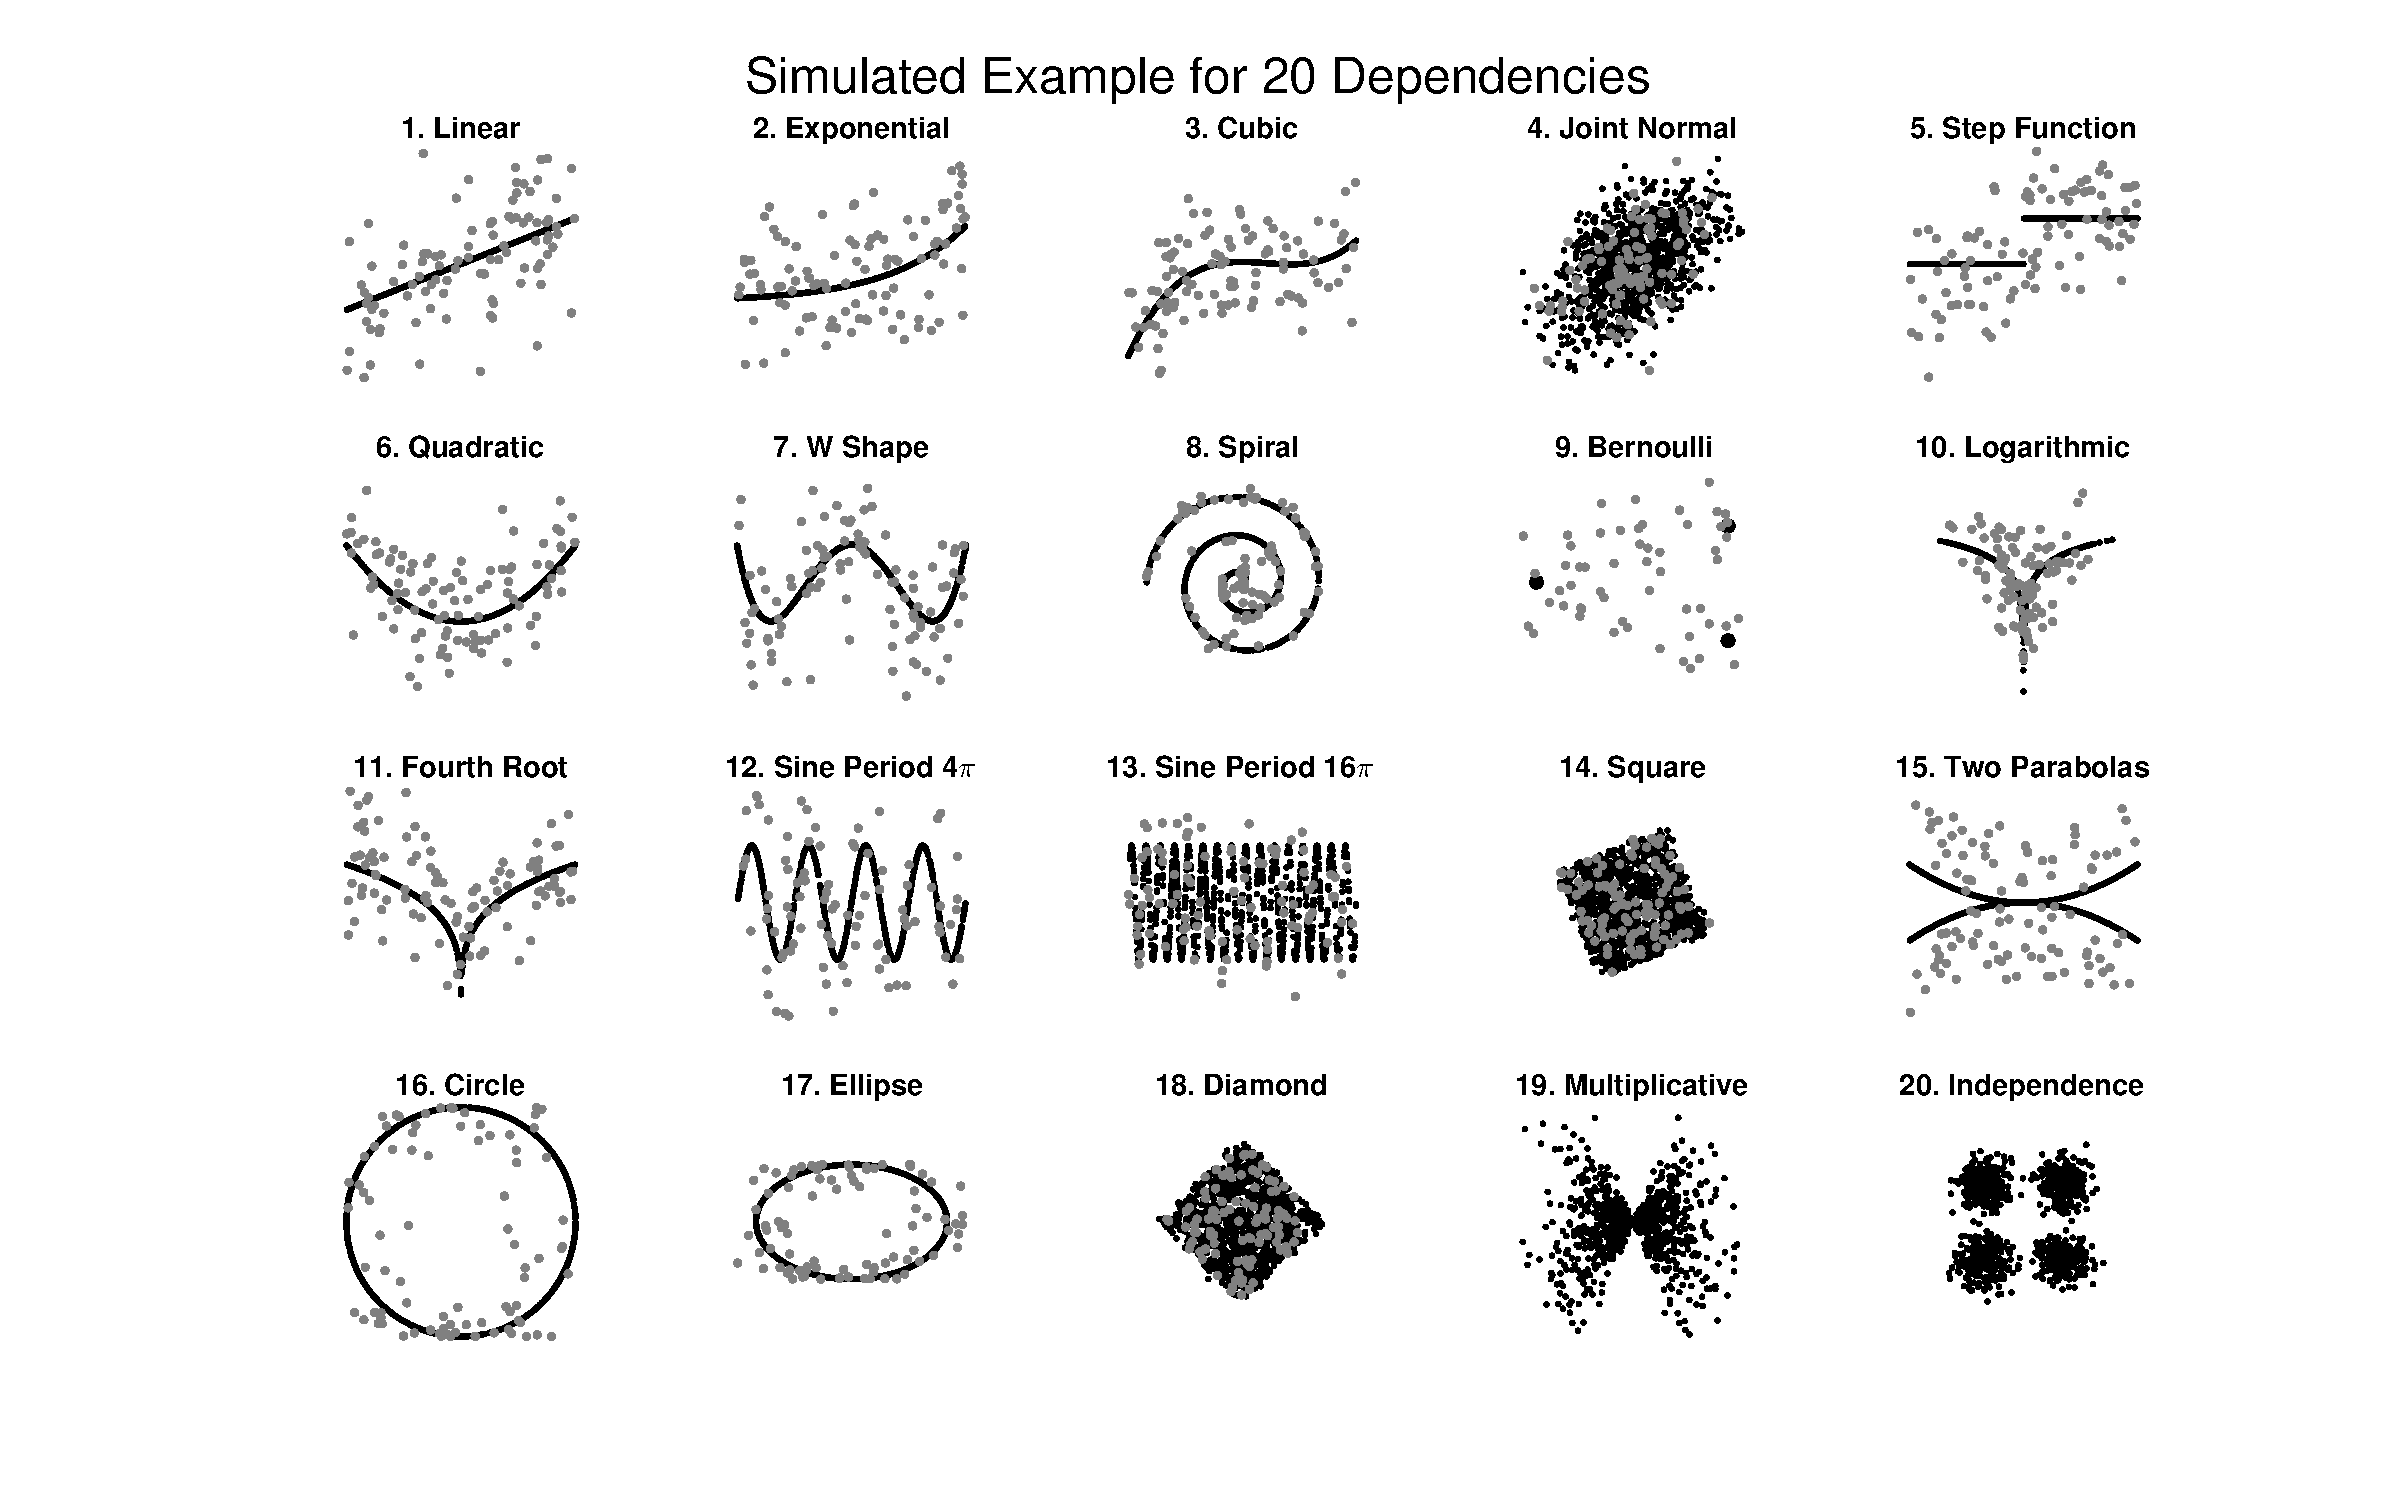
\includegraphics[trim={5cm 0 3.5cm 0},clip, width=1.0\textwidth]{../Figures/FigSimVisual.pdf}
\caption{Visualization of the $20$ dependencies for one-dimensional simulations. For each, we sampled $n=100$ points with noise to show the actual sample data used testing (gray dots). For comparison purposes, we also sampled $n=1000$ points without noise (c=1) to highlight each underlying dependency (black dots).
}
\label{f:dependencies}
\end{figure}



\begin{figure}[htbp]
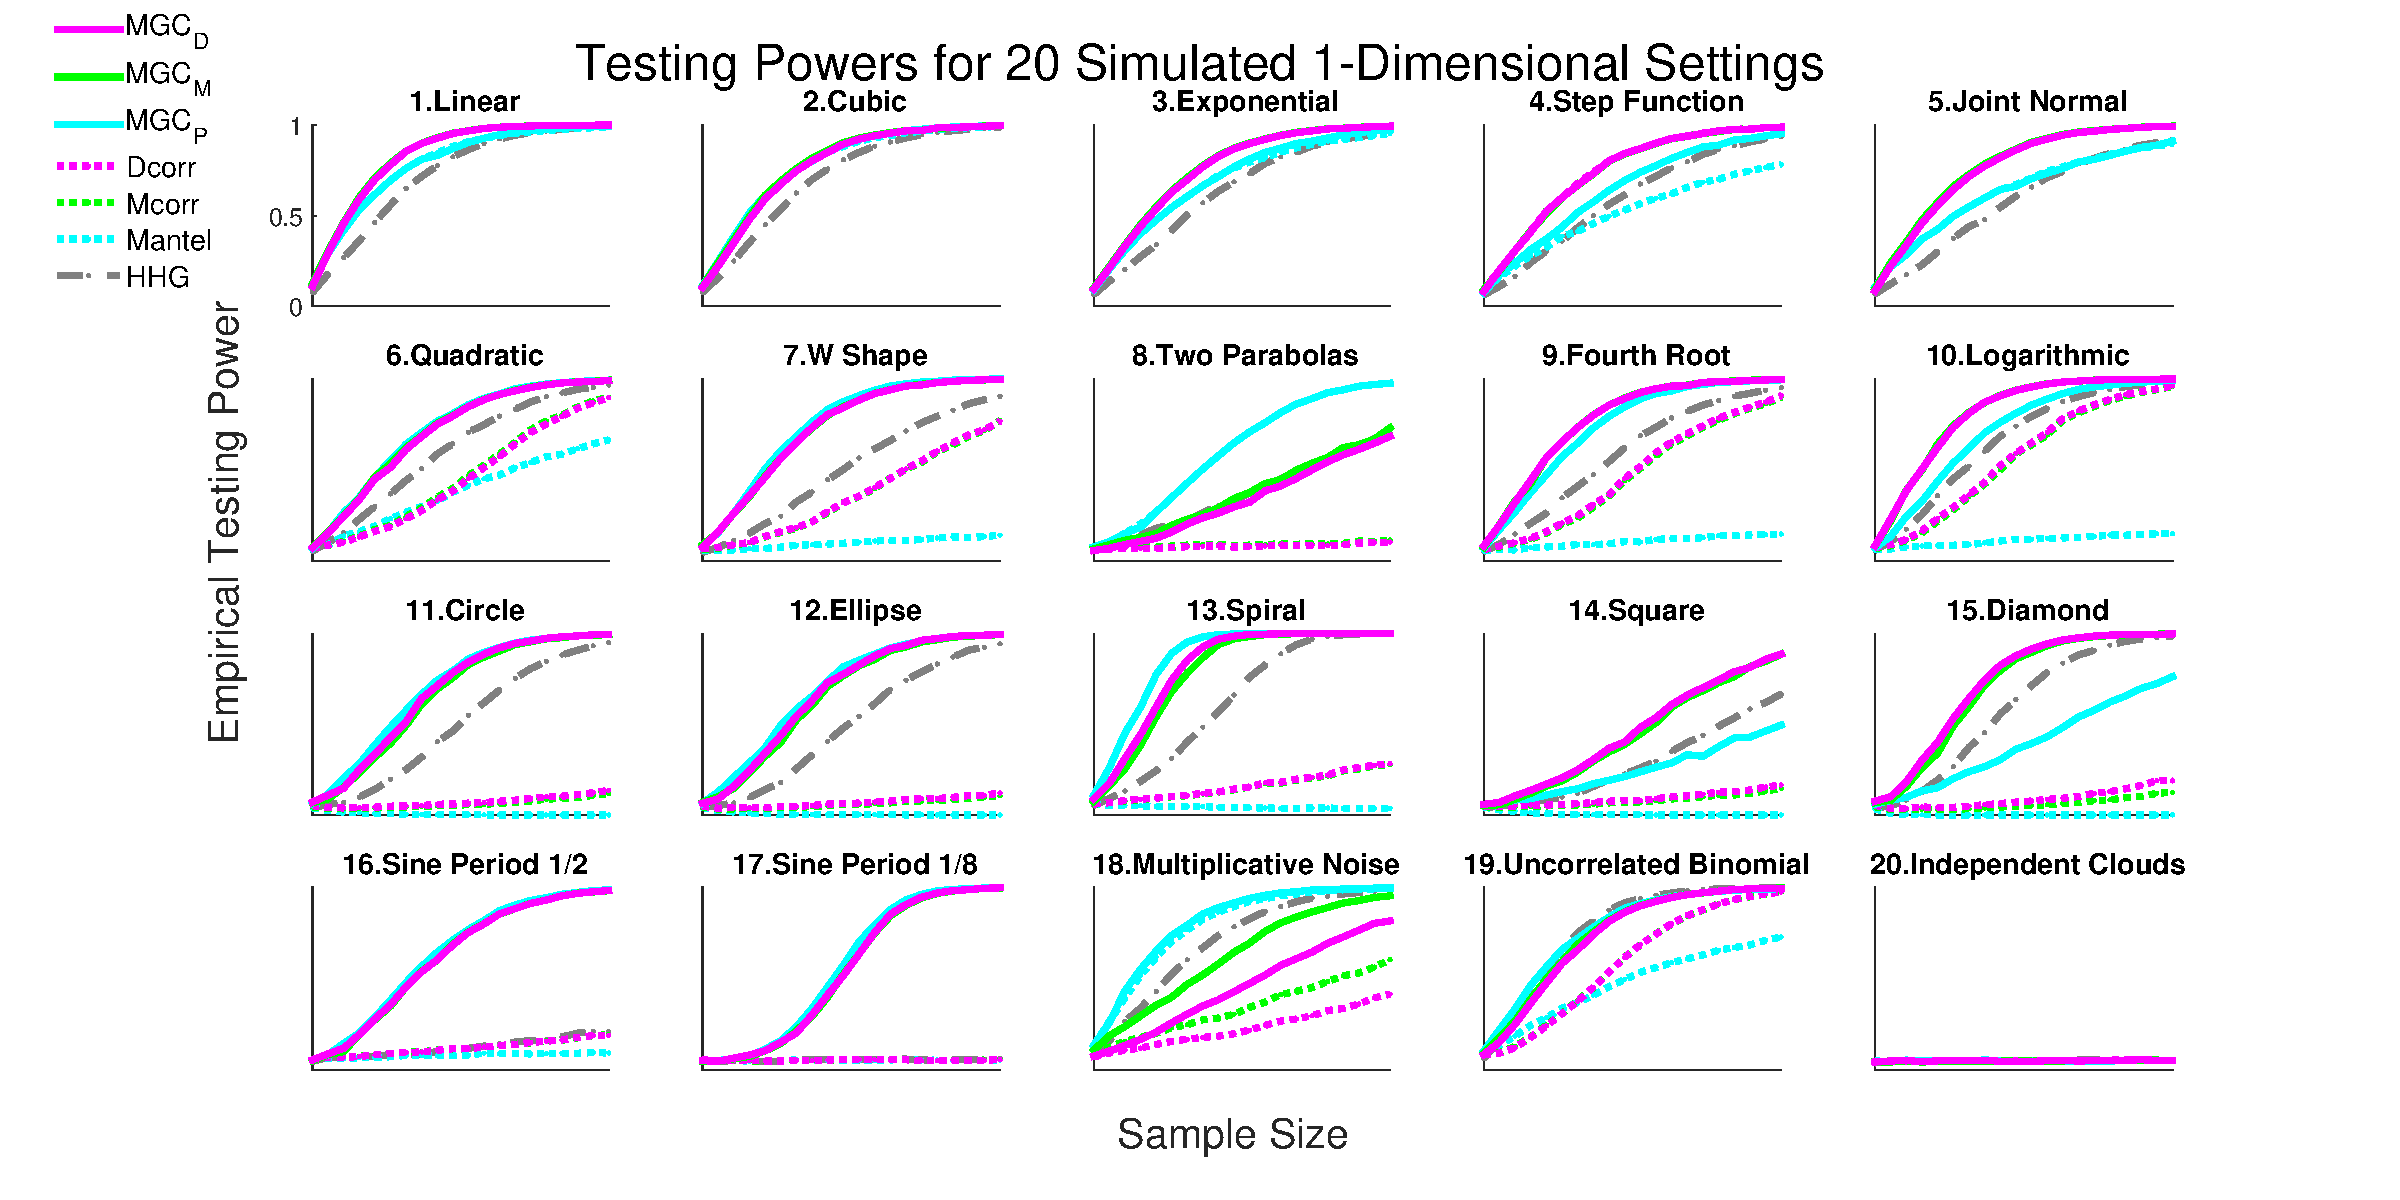
\includegraphics[width=1.0\textwidth]{../Figures/Fig1DPowerAll.pdf}
\caption{
Powers of different methods for $20$ different one-dimensional dependence structures, estimated by the empirical distributions of the test statistics under the null and the alternative.
 % on the basis of $10$,$000$ Monte-Carlo replicates. $2$,$000$ additional MC replicates are used for optimal scale estimation for \Mgc.
This figure includes seven different tests: \Mantel, \Dcorr, and \Mcorr (magenta dotted, dashed, and solid lines, respectively), as well as their corresponding \Mgc~counterparts, \Mgcp, \Mgcd, \Mgcm (green with same line styles), as well as \Hhg (gray).
Each panel shows empirical testing power on the abscissa at a significance level $\alpha=0.05$, and sample size on the ordinate.
\Mgc~empirically achieves similar or better power than the previous state of the art approaches for all sample sizes on almost all problems.}
\label{f:1DAll}
\end{figure}

\begin{figure}[htbp]
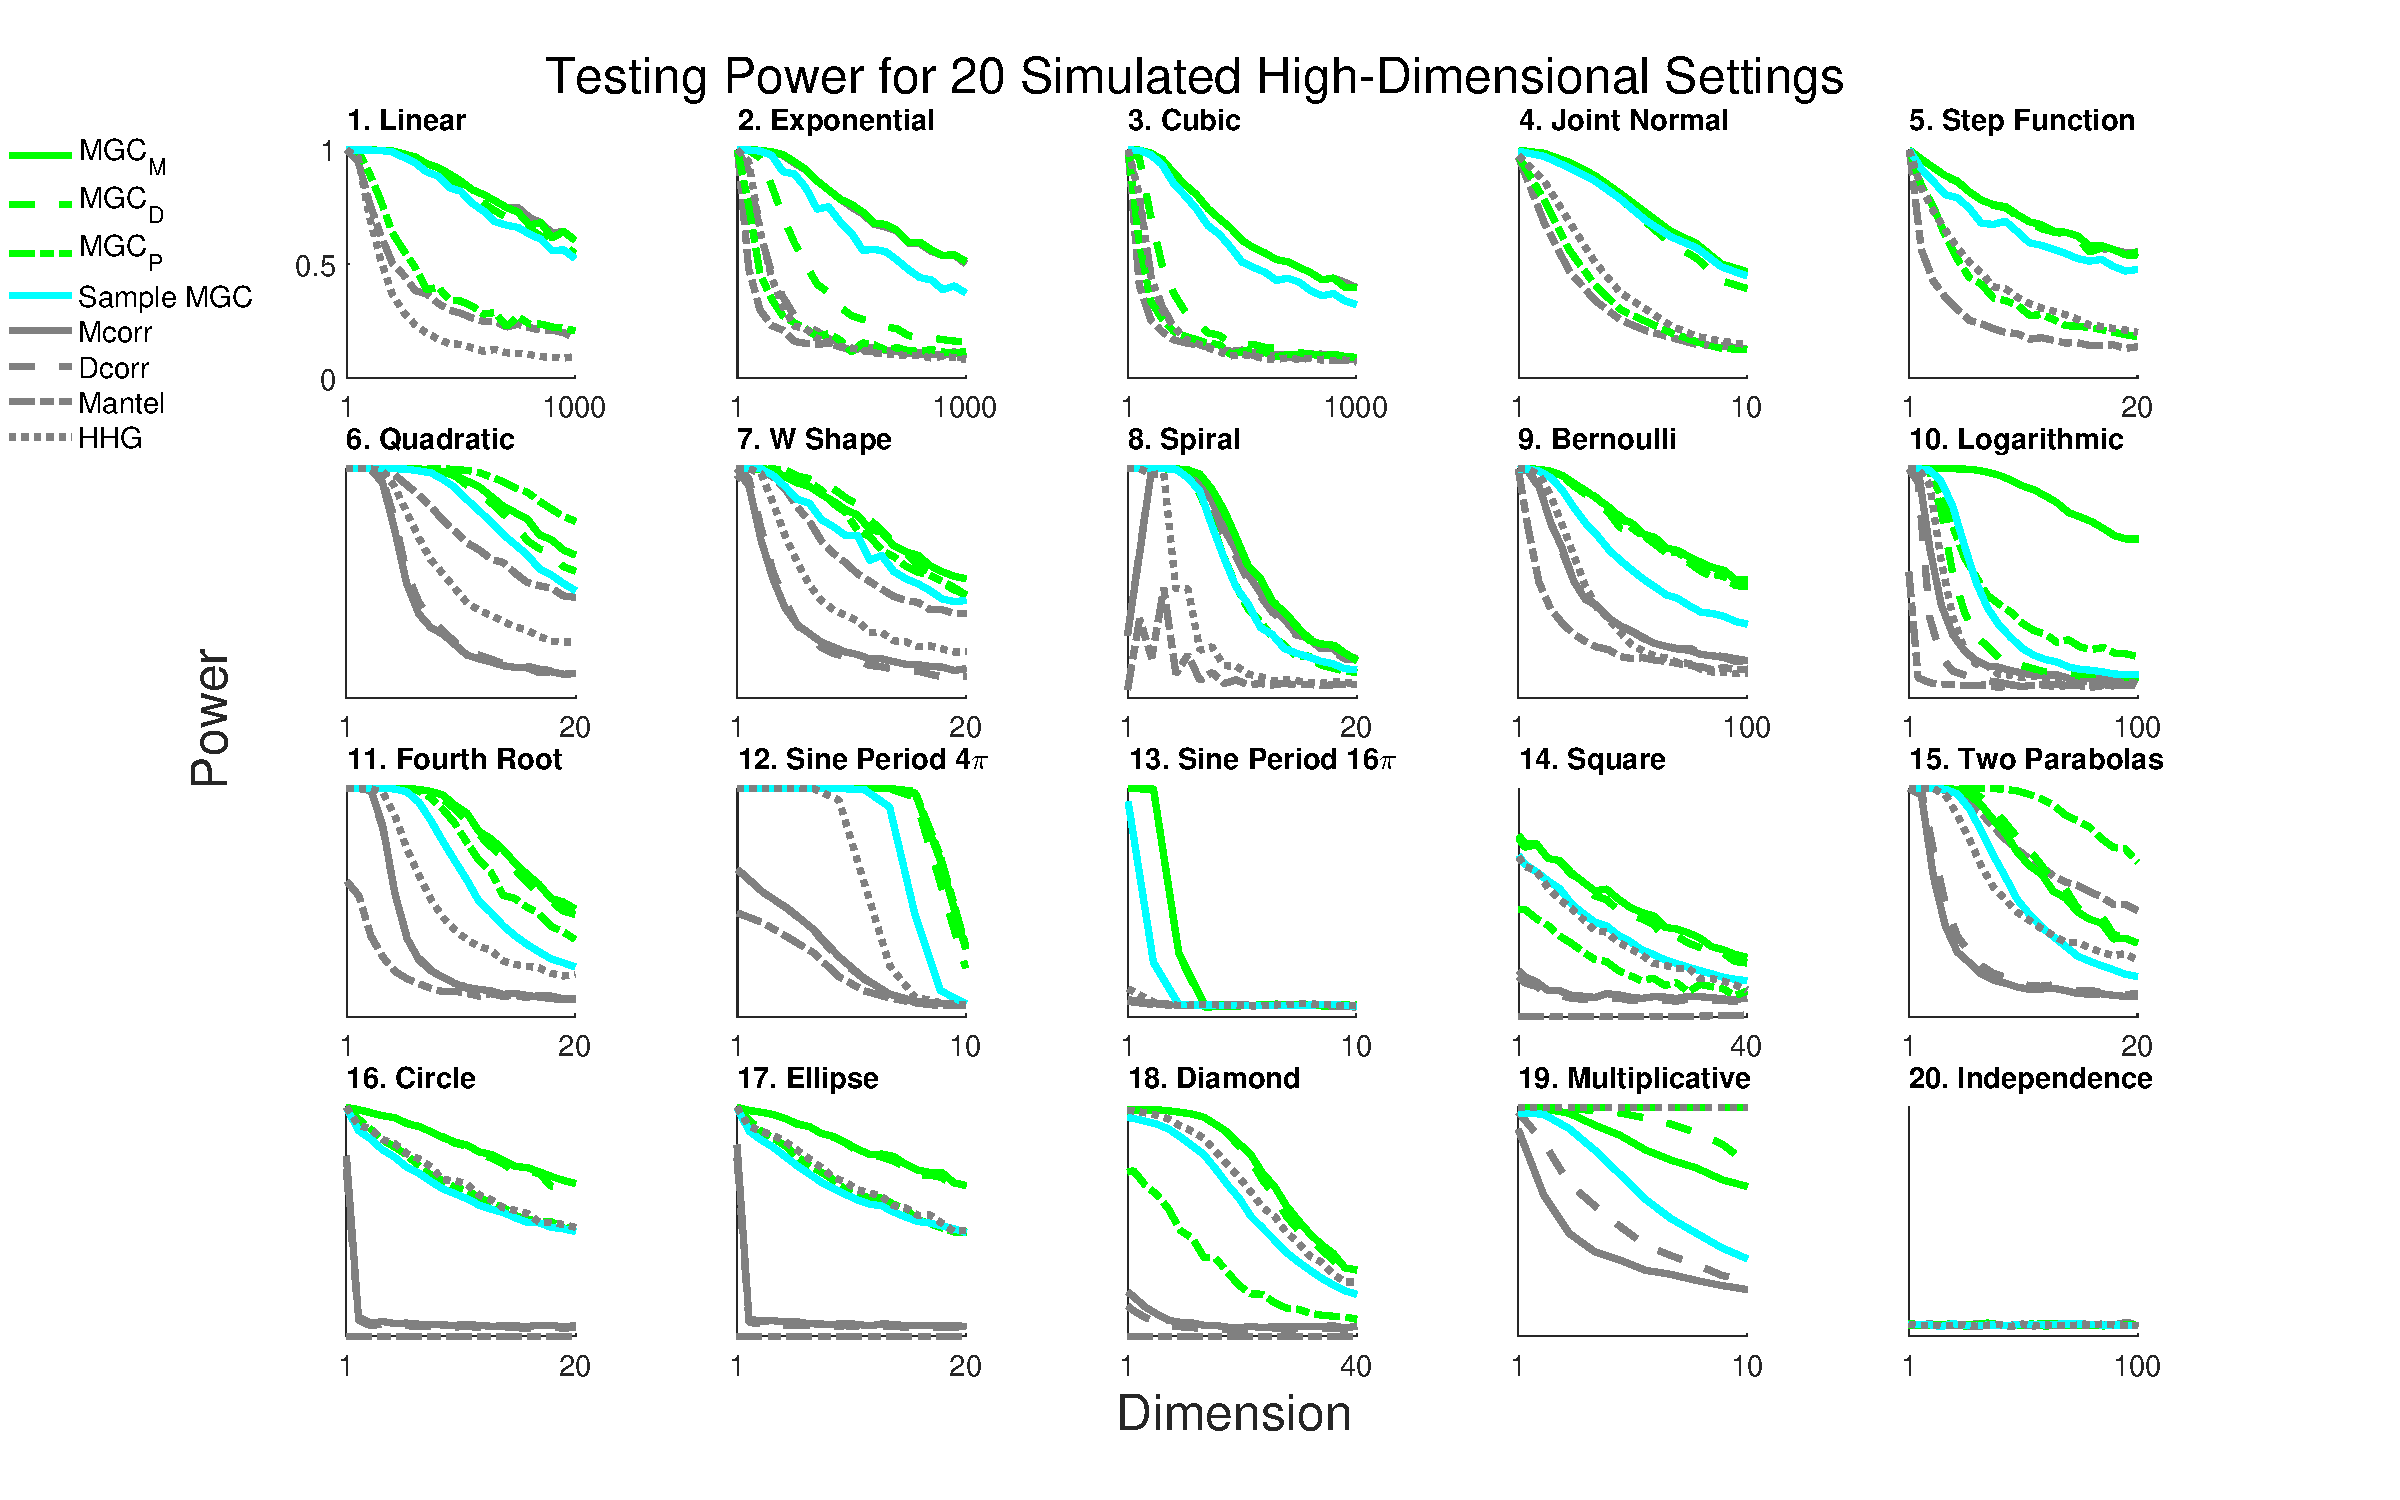
\includegraphics[width=1.0\textwidth]{../Figures/FigHDPowerAll.pdf}
\caption{
Same as Figure~\ref{f:nD} in main text, but with all seven methods compared. Note that oracle \Mgc~dominates the other approaches by always being as powerful or more so, regardless of dimensionality and distribution. \Mgc~is always plotted ``on top'' of the global variants, therefore, some of the global variants are not always visible from the display.}
\label{f:nDAll}
\end{figure}


\begin{figure}[htbp]
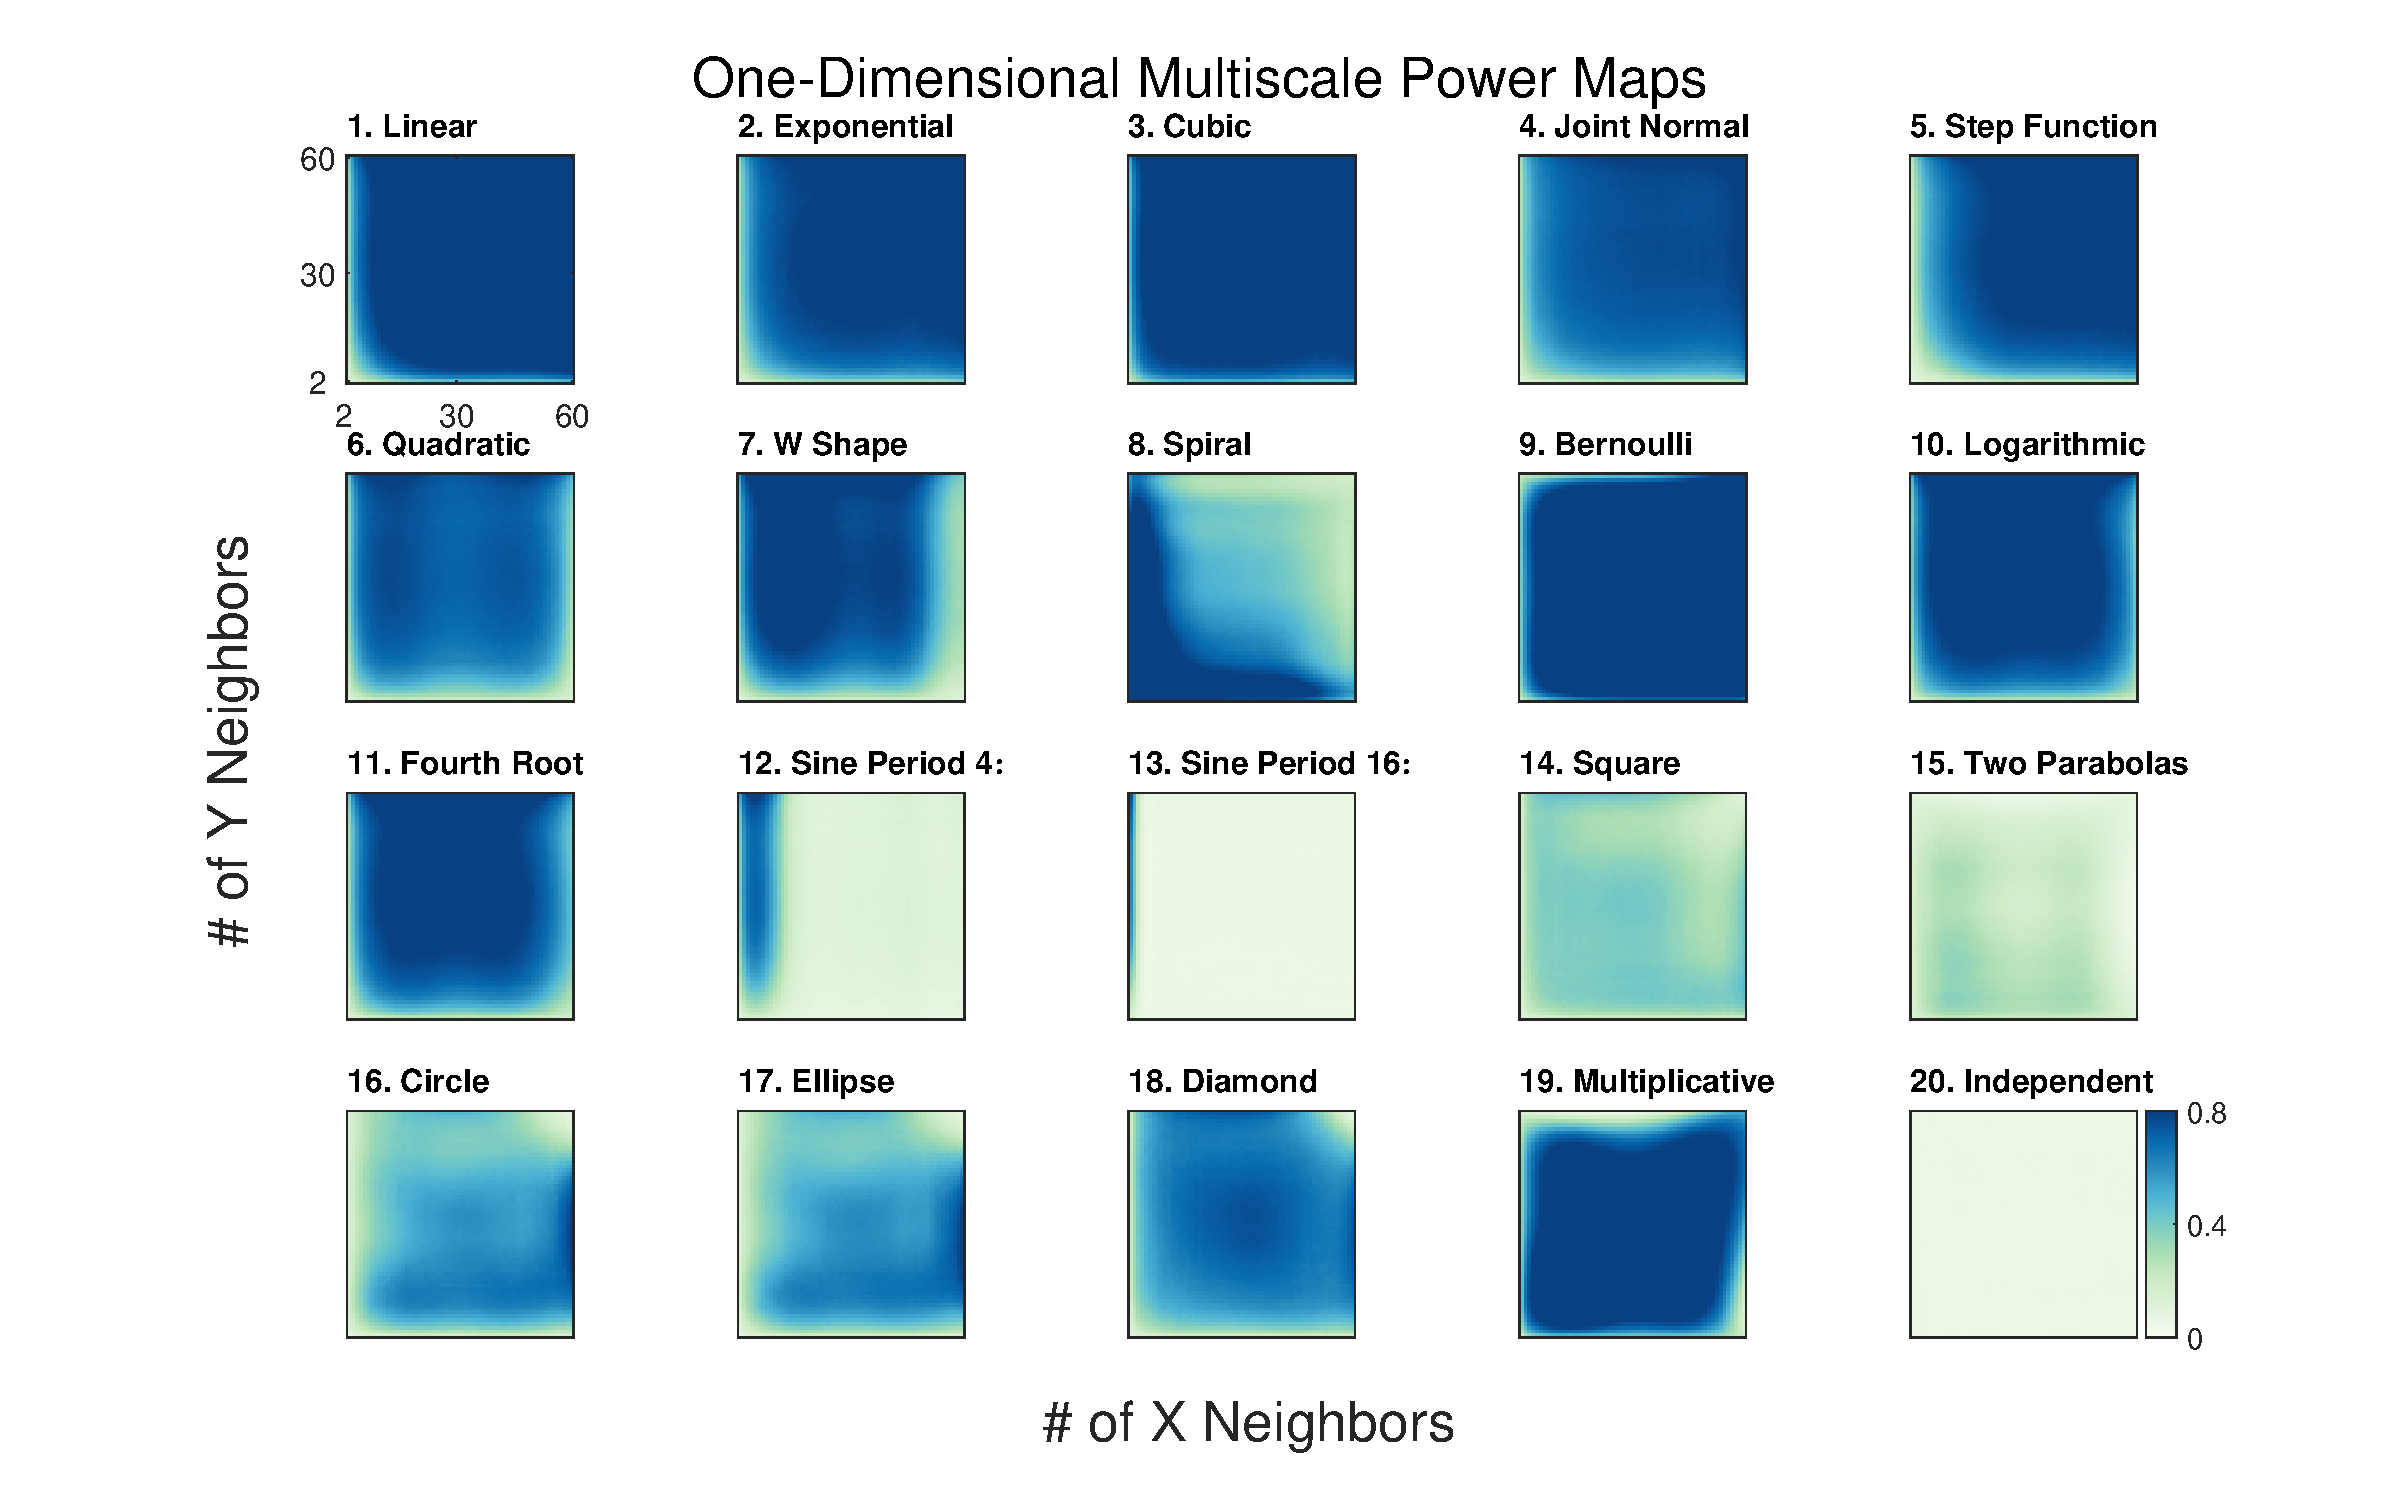
\includegraphics[width=1.0\textwidth]{../Figures/Fig1DHeat.pdf}
\caption{Multiscale Power Maps indicating the influence of neighborhood size on \Mgc~testing power, for the one-dimensional simulations in Figure~\ref{f:1DAll}. For each simulation,  the sample size is $n=60$, and the significance level is $\alpha=0.05$. For the (nearly) linear settings, the global scales achieve optimal power.  However, for the other nonlinear dependence settings, local scales always outperform the global setting.}
\label{f:powermaps1}
\end{figure}

\begin{figure}
  \centering
  \begin{tabular}{@{}p{0.4\linewidth}@{\quad}p{0.4\linewidth}@{}}
	  \centering
    \subfigimg[width=\linewidth]{A}{../Figures/Fig1DPerm} &
    \subfigimg[width=\linewidth]{B}{../Figures/FigHDPerm}
  \end{tabular}
\caption{%
Comparing the sample \Mgc~powers to the powers of oracle \Mgc, \Mcorr, and \Hhg, for all one-dimensional and high-dimensional simulations except the independent clouds. We plot the power difference between each of oracle \Mgc, \Mcorr, and \Hhg, to the sample \Mgc. Thus, values larger than zero indicate \emph{better}  than \Mgc~power estimated from p-value maps as we do for real data, and values smaller than zero indicate \emph{worse}.
(A) One-dimensional simulations, where $n=60$ and $D=1$.
(B) High-dimensional simulations, where $n=100$ and the dimension is chosen as in Figure~\ref{f:powermaps}.
While sometimes less than the optimal \Mgc~powers computed from multiscale power maps, sample \Mgc~powers estimated from the p-value maps still dominate  \Mcorr~and often improve upon \Hhg's powers, especially in the high-dimensionality settings.}
\label{f:simPerm}
\end{figure}




\clearpage
\section{Dependence Measures}
\label{appen:methods}

In this section, we review the \Mantel~test, distance correlation (\Dcorr), modified distance correlation (\Mcorr),  and  \Hhg. Note that for \Dcorr~and \Mcorr, we implement them in a slightly different but equivalent way from the original definition.  Moreover, as will be explained in more detail below, for each global generalized correlation test (including \Mantel, \Dcorr, and \Mcorr) we have constructed a multiscale variant, called \Mgcp, \Mgcd, and \Mgcm, respectively.  Unless otherwise specified, when we write \Mgc, we will always mean \Mgcm.

\subsection{(Global) \Mantel~Test}
\label{appen:mantel}
Given the Euclidean distance matrices $\tilde{A}$ and $\tilde{B}$, let  $A=\tilde{A}$, $B=\tilde{B}$, $\bar{a}=\frac{1}{n(n-1)}\sum_{i \neq j}^{n}(a_{ij})$ and similarly for $\bar{b}$.
The \Mantel~coefficient \cite{Mantel1967} is defined as
\begin{equation*}
\Mantel(X,Y)=\frac{\sum_{i \neq j}^{n}(a_{ij}-\bar{a})(b_{ij}-\bar{b})}{\sqrt{\sum_{i \neq j}^{n}(a_{ij}-\bar{a})^2 \sum_{i \neq j}^{n}(b_{ij}-\bar{b})^2}}.
\end{equation*}
Then the \Mantel~test is carried out by the permutation test.

Unlike distance correlation and \Hhg, the \Mantel~test is not consistent against all dependent alternatives, but it has been a very popular method in biology and ecology, possibly due to its simplicity and effectively. One can observe from Figure~\ref{f:nDAll} and ~\ref{f:1DAll} that global \Mantel~is sub-optimal relative to much more recently proposed tests (\Mantel~was proposed in 1967, \Dcorr~was not proposed until about 40 years later), and appears to be not consistent for many dependencies. Nonetheless,  \Mgcp~achieves comparable performances as other variants of \Mgc, which implies that \Mgcp~may be consistent against most, if not all dependent alternatives.

\subsection{(Global) Distance Correlation}
\label{appen:dcorr}
Given two distance matrices $\tilde{A}$ and $\tilde{B}$ of the sample data $X$ and $Y$, the sample distance covariance is defined by doubly centering the distance matrices:
\begin{equation*}
\label{dcovEqu}
dcov(X,Y)=\frac{1}{n^2}\sum_{i,j=1}^{n}a_{ij}b_{ij},
\end{equation*}
where $A=H\tilde{A}H$, $B=H\tilde{B}H$ with $H=I_{n}-\frac{J_{n}}{n}$, $I_n$ the $n \times n$ identity matrix (ones on the diagonal, zeros elsewhere)  and $J_n$ the $n \times n$ matrix of all ones. The sample distance variance is defined as
\begin{align*}
dvar(X) &=\frac{1}{n^2}\sum_{i,j=1}^{n}a_{ij}^{2},\\
dvar(Y) &=\frac{1}{n^2}\sum_{i,j=1}^{n}b_{ij}^{2},
\end{align*}
and the sample distance correlation equals
\begin{equation*}
\Dcorr(X,Y)=\frac{dcov(X,Y)}{\sqrt{dvar(X) \cdot dvar(Y)}}.
\end{equation*}

It is shown in \cite{SzekelyRizzoBakirov2007} that as $n \rightarrow \infty$, $\Dcorr(X,Y) \rightarrow \Dcorr(\mb{x},\mb{y}) \geq 0$, where $\Dcorr(\mb{x},\mb{y})$ denotes the population distance correlation between the underlying random variable $\mb{x}$ and $\mb{y}$. The population distance correlation is defined by the characteristic functions, which is zero if and only if $\mb{x}$ and $\mb{y}$ are independent. Thus the sample distance correlation is a consistent statistic for testing independence, i.e., the testing power $\beta_{\alpha}(\Dcorr(X,Y))$
converges to unity as $n$ increases, at any type $1$ error level $\alpha$. Note that all of $dcov, dvar$, \Dcorr~are always non-negative; and the consistency result assumes finite second moments of $\mb{x}$ and $\mb{y}$, which holds for a family of metrics not limited to the Euclidean distance \cite{Lyons2013}. Also note that the \Dcorr~above is actually the square of distance correlation in \cite{SzekelyRizzoBakirov2007}, but for ease of presentation the square naming is dropped here.

Alternatively, calculating the distance covariance by $A=H\tilde{A}$ and $B=\tilde{B}H$ gives the same statistic for distance covariance, i.e., instead of using doubly centered distance matrices, it is the same to singly center one distance matrix by row and the other distance matrix by column.
\begin{lem}
The distance covariance $dcov(X,Y)$ is the same under single centering (i.e., $A=H\tilde{A}$ and $B=\tilde{B}H$) and double centering (i.e., $A=H\tilde{A}H$ and $B=H\tilde{B}H$), where $\tilde{A}$ and $\tilde{B}$ are the Euclidean distance matrices of $X$ and $Y$, and $H$ is the centering matrix. 

Moreover, the permutation p-value of global \Dcorr~is the same under single centering and double centering, so is the testing power.

The above also holds for \Mcorr~asymptotically.
\end{lem}
Our \Mgcd is in fact based on this single-centered \Dcorr, which is more advantageous than \Mgc based on double-centered \Dcorr (shown in Appendix~\ref{appen:mgc}). And the proofs of all lemmas are in Appendix~\ref{appen:proofs}.


\subsection{(Global) Modified Distance Correlation}
\label{appen:mcorr}
In case of high-dimensional data where the dimension $D$ or $D_y$ increases with the sample size $n$, the sample distance correlation may no longer be appropriate. For example, even for independent Gaussian distributions, $\Dcorr(X,Y) \rightarrow 1$ as $D, D_y \rightarrow \infty$, which may severally impair the testing power of sample \Dcorr~in high-dimensional simulations.

The modified distance correlation is proposed in \cite{SzekelyRizzo2013a} to tackle   \Dcorr's bias in high-dimensional settings. Denote the Euclidean distance matrices as $\tilde{A}$ and $\tilde{B}$, the doubly centered distance matrices as $\hat{A}$ and $\hat{B}$.  \Mcorr~defines $A$ by modifying the entries of $\hat{A}$ by
\[a_{ij} = \left\{
  \begin{array}{lr}
    \hat{a}_{ij}-\frac{\tilde{a}_{ij}}{n}, & \mbox{ if } i \neq j, \\
    \frac{1}{n}\sum_{j}\tilde{a}_{ij}-\frac{1}{n^2}\sum_{ij}\tilde{a}_{ij}, &\mbox{ if } i = j,
  \end{array}
\right.
\]
and  $B$ modifies the entires of $\hat{A}$ similarly.
The modified distance covariance is defined as
\begin{equation*}
mcov(X,Y)=\frac{n}{(n-1)^2(n-3)}\left(\sum_{i \neq j}^{n}a_{ij}b_{ij}-\frac{2}{n-2}\sum_{j=1}^{n}a_{jj}b_{jj}\right),
\end{equation*}
$mvar(X)$ and $mvar(Y)$ are similarly defined as well.

If $mvar(X) \cdot mvar(Y) \leq 0$, the modified distance correlation is set to $0$ (negativity can only occur when $n\leq 2$, equality can only happen in some special cases); otherwise it is defined as
\begin{equation*}
\Mcorr(X,Y)=\frac{mcov(X,Y)}{\sqrt{mvar(X) \cdot mvar(Y)}}.
\end{equation*}

It is shown in \cite{SzekelyRizzo2013a} that $\Mcorr(X,Y)$ is an unbiased estimator of the population distance correlation $\Dcorr(\mb{x},\mb{y})$ for all $D, D_y, n$; and \Mcorr~is approximately normal even if $D,D_y \rightarrow \infty$. Thus it is a consistent statistic for testing independence, and may work better than \Dcorr~under high-dimension dependencies.

Similar to the alternative implementation of \Dcorr, we can also use singly centered distance matrices for $\hat{A}$ and $\hat{B}$ in defining \Mcorr without alter the theoretical advantages of original \Mcorr. We further set $A_{ii}=B_{ii}=0$ for all $i$, which simplifies the expression of \Mcorr~and is asymptotically equivalent for testing. 
Thus we use the single-centered \Mcorr~with the simplified diagonal modification for computational expediency and simplicity.

%Also note that when there exists repeating points, it is necessary to set $a_{ij}=a_{jj}$ for repeating points during global/local mcorr computation, or exclude repeating observation before-hand, otherwise the diagonal adjustment of mcorr may lose its effect for adjusting high-dimensional bias.

\subsection{Heller, Heller \& Gorfine (\Hhg)}
\label{appen:hhg}

The \Hhg~statistic applies Pearson's chi-square test to ranks of distances within each column, and is shown to be better than many global tests including \Dcorr~under common nonlinear dependencies in \cite{GorfineHellerHeller2012, HellerGorfine2013}. Like \Dcorr~and \Mcorr, \Hhg~is distance-based and consistent, but not in the form of the generalized correlation coefficient; and like our \Mgc, it makes use of the rank information, but in a different manner.

Given the Euclidean distance matrices $\tilde{A}=\{\tilde{a}_{ij}\}$ and $\tilde{B}=\{\tilde{b}_{ij}\}$, we denote
\begin{align*}
H_{11}(i,j) &= \sum_{q=1,q\neq i,j}^{n}I(\tilde{a}_{iq} \leq \tilde{a}_{ij})I(\tilde{b}_{iq} \leq \tilde{b}_{ij}) \\
H_{12}(i,j) &= \sum_{q=1,q\neq i,j}^{n}I(\tilde{a}_{iq} \leq \tilde{a}_{ij})I(\tilde{b}_{iq} > \tilde{b}_{ij}) \\
H_{21}(i,j) &= \sum_{q=1,q\neq i,j}^{n}I(\tilde{a}_{iq} > \tilde{a}_{ij})I(\tilde{b}_{iq} \leq \tilde{b}_{ij}) \\
H_{22}(i,j) &= \sum_{q=1,q\neq i,j}^{n}I(\tilde{a}_{iq} > \tilde{a}_{ij})I(\tilde{b}_{iq} > \tilde{b}_{ij}),
\end{align*}
and the \Hhg~statistic is defined as
\begin{align*}
\Hhg(X,Y) &= \sum_{i=1,j\neq i}^{n} \frac{(n-2)(H_{12}(i,j)H_{21}(i,j)-H_{11}(i,j)H_{22}(i,j))^2}{H_{1 \cdot}(i,j)H_{2 \cdot}(i,j)-H_{\cdot 1}(i,j)H_{\cdot 2}(i,j)},
\end{align*}
where $H_{1 \cdot}=H_{11}+H_{12}$, $H_{2 \cdot}=H_{21}+H_{22}$, $H_{\cdot 1}=H_{11}+H_{21}$, and $H_{\cdot 2}=H_{12}+H_{22}$. Thus \Hhg~is structurally different from all previous distance-based correlations, and cannot be conveniently expressed by Equation~\ref{generalCoef}.

The permutation test using the \Hhg~statistic is consistent against all dependent alternatives. In our numerical simulations, \Hhg~has relatively low power  when testing against high-dimensional and noisy linear dependencies, but is often more advantageous than global correlations under nonlinear dependencies, which makes it a strong competitor in general.

\subsection{Multiscale Generalized Correlation (\Mgc)}
\label{appen:mgc}
For any generalized correlation coefficient, its local correlations can be directly implemented as in Equation~\ref{localCoef}, by plugging in the respective $a_{ij}$ and $b_{ij}$ from Equation~\ref{generalCoef} and rank-truncating  the distance matrices  as in Equation~\ref{localCoef2}. 

In particular, \Mantel~sets $a_{ij}$ and $b_{ij}$ as the respective entry of $\tilde{A}$ and $\tilde{B}$ (the Euclidean distances). \Dcorr~lets $a_{ij}$ and $b_{ij}$ be the respective matrix entry of $A$ and $B$ (the doubly centered distance matrices), then the sample means $\bar{a}, \bar{b}$ are automatically $0$. \Mcorr~slightly modifies $a_{ij}$ and $b_{ij}$ of \Dcorr~to adjust their high-dimensional bias. 

As discussed already, our \Mgcd~and \Mgcm~are based on single centering throughout, not only because single centering is equivalent to double centering for the global correlation, but also because single centering is consistent in preserving ranks while double centering is not, e.g., the ranks by sorting $\tilde{A}$ within each column are exactly the same as the column ranks of $H\tilde{A}$, which are different from the column ranks of $H\tilde{A}H$. 

Note that we defined the rank-truncated comparisons differently for $\mt{a}_{ij}^k$ and $\mt{b}_{ij}^l$: $\mt{a}_{ij}^k$ is defined based on ranks within each column, while $\mt{b}_{ij}^l$ is defined based on ranks within each row. By doing so, the ranks are consistent between $\tilde{Z}$ and $Z$ for either $Z=A,B$, and the resulting local correlations are always symmetric even if $A$ and $B$ are not symmetric.

\begin{lem}
Each local correlation $\G^{kl}$ is always symmetric regardless of the symmetry of $A$ or $B$. Namely for any $k,l$, 
\begin{align*}
\G^{kl}(X,Y)=\G^{lk}(Y,X).
\end{align*}

Furthermore, the column ranks of $\tilde{A}$ are preserved in $A$ under single centering but not double centering; similarly the row ranks of $\tilde{B}$ are preserved in $B$ under single centering.
\end{lem}
Therefore local correlations are more faithful in excluding far-away observations that exhibit insignificant dependency, when \Mgc~is implemented by single centering.

Generally, there are a total of $\max(R(a_{ij})) \times \max(R(b_{ij}))$ local correlations, which equals $n^2$ when there exists no repeating values of \mbx~or \mby. Note that we use minimal ranks in sorting when ties occur, which guarantees that all local correlations are indexed consecutively. Alternatively, one may add a very small amount of white noise to break all ties, like in our real data experiment.

Among all possible local correlations, \Mgc~picks the optimal local correlation. Optimal scales always exist,  is distribution dependent, and are often non-unique. Among all local correlations, it suffices to exclude $\G^{1l}$ and $\G^{k1}$ for testing and optimal scale estimation: since $\G^{1l}=\G^{k1}=\G^{11}$, they do not include any neighbor other than each observation itself, merely count the diagonal terms in the distance matrices, and are not meaningful for the testing purpose.

% See Appendix \ref{appen:algorithms} for details of all relevant algorithms.

\section{\Mgc~Algorithms and Testing Procedures}
\label{appen:tests}
In this section we elaborate on the algorithms for computing local correlation and \Mgc, as well as their testing procedures in simulations and real data experiment.

Five algorithms are presented in Appendix~\ref{appen:algorithms}: Algorithm~\ref{alg:1scale} directly computes the local correlation coefficient at a given scale $(k,l)$, for a given choice of a global correlation coefficient.
Algorithm~\ref{alg:all_scales} provides an efficient method to compute all local correlations simultaneously, in the same running time complexity as computing one local correlation. Algorithm~\ref{alg:pval} computes the p-values of all local correlation by the random permutation test. 
Algorithm~\ref{alg:power} estimates the testing powers of all local statistics using a known or estimated joint distribution, which can be used to more accurately estimate the optimal scales and the testing power for \Mgc. 
Algorithm~\ref{alg:best_scale} approximates the optimal scales for \Mgc~by finding a consecutive region of scales with significant and monotonically decreasing (along either the row or column indices) p-values, and 
outputting the approximated p-value and all optimal scales for the sample \Mgc. More detailed discussions regarding the optimal scales approximation is offered in Appendix~\ref{appen:diss}.
%Algorithm~\ref{alg:best_scale_aux} is an auxiliary function of Algorithm~\ref{alg:best_scale}, which validates that the consecutive region should consists of rectangles.

\subsection{Algorithms}
\label{appen:algorithms}
All algorithms are implemented in Matlab and R with the algorithm shown below. For ease of presentation, we assume there are no repeating observations of \mbx~or \mby, and assume \Dcorr~is the global correlation.

\begin{algorithm}
\caption{Local Correlation Computation for One Scale. This algorithm runs in $O(n^2)$ once the rank information is provided, which is suitable for \Mgc~computation if an optimal scale is already estimated. But it would take $O(n^4)$ if used to compute all local correlations. Note that for the default \Mgc~implementation by single centering, the centering function centers $\tilde{A}$ by column and $\tilde{B}$ by row, and the sorting function sorts $\tilde{A}$ within column and $\tilde{B}$ within row.}
\label{alg:1scale}
\begin{algorithmic}[1]
\Require A pair of distance matrices $(\tilde{A},\tilde{B}) \in \Real^{n \times n} \times \Real^{n \times n}$, and the given local scale $(k,l) \in \Real \times \Real$.
\Ensure The local correlation coefficient $\G^{kl} \in [-1,1]$ at the given $(k,l)$.
\Function{LocalCorr}{$\tilde{A}$,$\tilde{B}$,$k$,$l$}
\State Initialize $\G^{kl}$, $V^{A}_{k}$, $V^{B}_{l}$, $E^{A}_{k}$, $E^{B}_{l}$ at $0$.
\Linefor{$Z:=A,B$}{$R^{Z}=\textsc{Sort}(\tilde{Z})$} \Comment{sort distances}
\Linefor{$Z:=A,B$}{$Z=\textsc{Center}(\tilde{Z})$}  \Comment{center distance matrices}
%\State $R^{B}=\textsc{Transpose}(R^{B})$ \Comment{row-wise ranks are used for second data}
%\State $B=\textsc{Transpose}(B)$ \Comment{row-wise ranks are used for second data}

\For{$i,j:=1,\ldots,n$}
\State $\G^{kl} \rto \G^{kl}+A_{ij}B_{ij}\mb{I}(R^{A}_{ij} \leq k)\mb{I}(R^{B}_{ij} \leq l)$ \Comment{update un-centered local distance covariance}
\Linefor{$Z:=A,B$}{$V^{Z}_{k} \rto V^{Z}_{k}+Z_{ij}^2\mb{I}(R^{Z}_{ij} \leq k)$} \Comment{update local distance variances}
\Linefor{$Z:=A,B$}{$E^{Z}_{k} \rto E^{Z}_{k}+Z_{ij}\mb{I}(R^{Z}_{ij} \leq k)$} \Comment{update sample means}
\EndFor

\State $\G^{kl} \rto \left(\G^{kl}-E^{A}_{k}E^{B}_{l}/n^2\right)/\sqrt{\left(V^{A}_{k}-{E^{A}_{k}}^2/n^2\right) \left(V^{B}_{l}-{E^{B}_{l}}^2/n^2\right)}$ \Comment{center and normalize} 
% the local covariances}

\EndFunction
\end{algorithmic}
\end{algorithm} 

\begin{algorithm}
\caption{Local Correlation Computation for All Scales. Once the distances are sorted, this algorithm computes all local correlations in $O(n^2)$. An important observation is that each product $a_{ij}b_{ij}$ is included in $\G^{kl}$ if and only if $(k,l)$ satisfies $k\leq R(a_{ij})$ and $l\leq R(b_{ij})$, so it suffices to iterate through $a_{ij}b_{ij}$ for $i,j=1,\ldots,n$, and add the product simultaneously to all $\G^{kl}$ whose scales are no more than $(R(a_{ij}),R(b_{ij}))$. To achieve the above, we iterate through each product, add it to $\G^{kl}$ at $(k,l)=(R(a_{ij}),R(b_{ij}))$ only (so only one local scale is accessed for each operation); then add up adjacent $\G^{kl}$ for $k,l=1,\ldots,n$. The same applies to all local covariances, variances and expectations.} %Thus all local correlations can be computed in $O(n^2)$, which has the same running time complexity as the global distance correlation. There are two additional overheads: sorting the distance matrices column-wise takes $O(n^2 \log n)$, and properly centering the distance matrices takes $O(n^2)$.}
\label{alg:all_scales}
\begin{algorithmic}[1]
\Require A pair of distance matrices $(\tilde{A},\tilde{B}) \in \Real^{n \times n} \times \Real^{n \times n}$.
\Ensure All local correlation coefficients $\G^{kl} \in [-1,1]^{n \times n}$ for $k,l=1,\ldots,n$.
\Function{LocalCorr}{$\tilde{A}$,$\tilde{B}$}
\State Initialize $C$ as a zero matrix of size $n \times n$; $V^{A}$, $V^{B}$, $E^{A}$, $E^{B}$ as zero vectors of size $n$.
\Linefor{$Z:=A,B$}{$R^{Z}=\textsc{Sort}(\tilde{Z})$}
%\State $R^{B}=\textsc{Transpose}(R^{B})$ 
\Linefor{$Z:=A,B$}{$Z=\textsc{Center}(\tilde{Z})$}

\For{$i,j:=1,\ldots,n$} \Comment{iterate through all local scales to calculate each term} 
\State $k \rto R^{A}_{ij}$
\State $l \rto R^{B}_{ij}$
\State $\G^{kl} \rto \G^{kl}+A_{ij}B_{ij}$
\State $V^{A}_{k} \rto V^{A}_{k}+A_{ij}^2$
\State $V^{B}_{l} \rto V^{B}_{l}+B_{ij}^2$
\State $E^{A}_{k} \rto E^{A}_{k}+A_{ij}$
\State $E^{B}_{l} \rto E^{B}_{l}+B_{ij}$
\EndFor

\For{$k:=1,\ldots,n-1$} \Comment{iterate through each scale again and add up adjacent terms} 
\State $\G^{1, k+1} \rto \G^{1, k}+\G^{1, k+1}$
\State $\G^{k+1,1} \rto \G^{k+1,1}+\G^{k+1,1}$
\Linefor{$Z:=A,B$}{$V^{Z}_{k+1} \rto V^{Z}_{k}+V^{Z}_{k+1}$}
\Linefor{$Z:=A,B$}{$E^{Z}_{k+1} \rto E^{Z}_{k}+E^{Z}_{k+1}$}
\EndFor

\For{$k,l:=1,\ldots,n-1$} 
\State $\G^{k+1,l+1} \rto \G^{k+1,l}+\G^{k,l+1}+\G^{k+1,l+1}-\G^{k,l}$
\EndFor

\For{$k,l:=1,\ldots,n$} 
\State $\G^{kl} \rto \left(\G^{kl}-E^{A}_{k}E^{B}_{l}/n^2\right)/\sqrt{\left(V^{A}_{k}-{E^{A}_{k}}^2/n^2\right) \left(V^{B}_{l}-{E^{B}_{l}}^2/n^2\right)}$
\EndFor
\EndFunction
\end{algorithmic}
\end{algorithm}

\begin{algorithm}
\caption{P-value Computation for All Local Correlations. This algorithm computes the p-values of all local correlation by the permutation test with $r$ random permutations, which takes $O(rn^2 \log n)$. $\pi$ denotes a random permutation, and $\tilde{B}(\pi,\pi)$ denotes the distance matrix with the observation label permuted. In the real data experiment we always set $r=10$,$000$.}
\label{alg:pval}
\begin{algorithmic}[1]
\Require A pair of distance matrices $(\tilde{A},\tilde{B}) \in \Real^{n \times n} \times \Real^{n \times n}$, the number of permutations $r$.
\Ensure The p-value matrix $P \in [0,1]^{n \times n}$ for all local distance correlations.
\Function{PermutationTest}{$\tilde{A}$,$\tilde{B}$,$r$}
\State $\G^{kl}=\textsc{LocalCorr}(\tilde{A},\tilde{B})$ \Comment{calculate the observed local correlations}
\For{$j:=1,\ldots,r$}
\State $\pi=\textsc{RandPerm}(n)$ \Comment{generate a random permutation of size $n$} 
\State $\G^{kl}_{0}[j]=\textsc{LocalCorr}(\tilde{A},\tilde{B}(\pi,\pi))$ \Comment{calculate the permuted test statistics}
\EndFor

\Linefor{$k,l:=1,\ldots,n$}{$P_{kl} \rto \sum_{j=1}^{r}(\G^{kl} \leq \G^{kl}_{0}[j])/r$}
\EndFunction
\end{algorithmic}
\end{algorithm}

\begin{algorithm}
\caption{Testing Powers Computation for All Local Correlations: this algorithm computes the testing powers of all local correlations. By repeatedly simulating samples by the joint distribution $f_{xy}$, sample data of size $n$ under the null and the alternative are generated for $r$ Monte-Carlo replicates. Then all sample local correlations under the null and the alternative are computed by Algorithm~\ref{alg:all_scales}, followed by estimating the testing power at each local correlation. The \Mgc~optimal scale can be found by selecting the scale that maximizes power, and it suffices to pick one optimal scale in case of ties. In the simulation we use $r=2$,$000$ MC replicates to estimate the optimal scale, and another $r=10$,$000$ MC replicates to estimate the power. The running time is $O(rn^2 \log n)$. This algorithm can be similarly adapted to training data, for which the alternative statistic can be computed from the training data while the null statistic can be computed by permutation. }
\label{alg:power}
\begin{algorithmic}[1]
\Require A joint distribution $f_{xy}$, the sample size $n$, the number of MC replicates $r$, and the type $1$ error level $\alpha$.
\Ensure The power matrix $\beta_{\alpha} \in [0,1]^{n \times n}$ for all local correlations, and the \Mgc~optimal scale $(k^{*},l^{*}) \in \Real \times \Real$.
\Function{TestingPowers}{$f_{xy}$,$n$, $r$,$\alpha$}
\For{$j:=1,\ldots,r$}
\Linefor{$i:=[n]$}{$(X^{1}_{i},Y^{1}_{i}) \stackrel{iid}{\sim} f_{xy}$, $X^{0}_{i} \stackrel{iid}{\sim} f_{x}$, $Y^{0}_{i} \stackrel{iid}{\sim} f_{y}$} 
\Linefor{$Z:=A,B$}{$\tilde{Z}_{1}=\textsc{Dist}(Z_{1})$, $\tilde{Z}_{0}=\textsc{Dist}(Z_{0})$} 
\State $\G^{kl}_{1}[j]=\textsc{LocalCorr}(\tilde{A}_{1},\tilde{B}_{1})$ \Comment{calculate all local correlations under the alternative}
\State $\G^{kl}_{0}[j]=\textsc{LocalCorr}(\tilde{A}_{0},\tilde{B}_{0})$ \Comment{calculate all local correlations under the null}
\EndFor

\For{$k,l:=1,\ldots,n$}
\State $c_{\alpha} \rto \textsc{Cdf}_{1-\alpha}(\G^{0}_{kl}[j],j \in [r])$ \Comment{get the critical value by the empirical distributions}
\State $\beta_{\alpha}^{kl} \rto \sum_{j=1}^{r}(\G^{1}_{kl}[j]>c_{\alpha}) / r$ \Comment{estimate the power}
\EndFor
\State $(k^{*},l^{*}) \rto \arg\max(\beta_{\alpha}^{kl})$ \Comment{find the optimal local scale}
\EndFunction
\end{algorithmic}
\end{algorithm}

\begin{algorithm}
\caption{Optimal Local Scales Approximation by P-values. This algorithm approximates the optimal scales $(k^{*},l^{*})$ from the p-values of consecutive local correlations, and outputs both the optimal scales and their corresponding \Mgc~p-value. If the global p-value is among the top $\beta$ percentile of all p-values, we take the global correlation directly. Otherwise we first check the monotonically decreasing of p-value map along the row and column, and return a binary matrix with a larger area; then we check a list of possible p-values from $\beta$ percentile onwards, and find the largest connected component (through adjacent scales of size at least $\theta n$) in the p-value map that are smaller than the candidate p-value and are monotonically decreasing. We take the candidate p-value as the approximated \Mgc~p-value only if the percentage of the component is at least $\theta$. The running time is $O(n^2)$; see Appendix~\ref{appen:diss} for more discussion. }
\label{alg:best_scale}
\begin{algorithmic}[1]
\Require The p-value matrix $P \in \Real^{n \times n}$ of all local correlations, and the significance level $\alpha$.
\Ensure The approximated \Mgc~optimal scales $(k^{*},l^{*})$, and the approximated \Mgc~p-value $p$.
\Function{MGCScaleVerify}{$P, \alpha$}
\State $p \rto 0.5$ \Comment{default p-value}
\State $\beta \rto 0.1$ \Comment{the percentile value to check, need to be in $[0,1)$}
\State $\theta \rto 0.02$ \Comment{the threshold to check connected component}
\If{$\sum_{kl}(P<P[n,n])/n^2<\beta$} 
\State $p \rto P[n,n]$ \Comment{use the global p-value when it is small enough among all p-values}
\State $[k^{*},l^{*}] \rto [n,n]$
\Else
\State $M=\textsc{Monotone}(P)$ \Comment{return a binary matrix of same size as $P$}
\State $\Gamma=\textsc{Prctile}(P,[\beta,2\beta,\ldots,1-\beta] )$ \Comment{get the candidate p-values by percentile}
\State $\Gamma=\textsc{Sort}([\Gamma, \alpha])$ \Comment{add $\alpha$ to the candidate p-value list}
\For{$\gamma \in \Gamma$}
\State $PR = \textsc{LargestComponent}((M==1) \& (P \leq \gamma),\left\lceil n\theta \right\rceil)$ 
\If{$\frac{\sum_{kl}PR_{kl}}{(n-1)^2}>\theta$}
\State $p \rto \gamma$;
\State $[k^{*},l^{*}] \rto \arg_{\{k,l\}} (PR_{kl}==1)$
\State break
\EndIf
\EndFor
\EndIf
\EndFunction
\end{algorithmic}
\end{algorithm}

\clearpage
\subsection{Discussions of Optimal Scale Estimation}
\label{appen:diss}
Evaluating \Mgc~requires estimating the optimal scales. Algorithm~\ref{alg:power} is used whenever the true distribution of the data in known or easy to estimate or multiple training data are available, which yields the oracl \Mgc. Otherwise, we shall approximate the optimal scale by Algorithm~\ref{alg:best_scale}. Once the optimal scale is determined, the testing power of \Mgc~for the given distribution can be quickly determined by Algorithm~\ref{alg:power}, and its p-value for testing on a particular data realization can be determined by Algorithm~\ref{alg:pval}.

On the other hand, the target of sample \Mgc~is to achieve similar powers as oracle \Mgc, as well as minimizing bias from noisy p-value. To achieve so, Algorithm~\ref{alg:best_scale} searches for a consecutive region that has monotonically decreasing p-values along either the row or column indices, and has p-values lower than the candidate p-value. If the connected component is large enough, the candidate p-value is used as the approximate \Mgc~p-value, with the region being the approximate optimal scale. The parameter $\theta$ is an important threshold to combat the bias, which can be increased or decreased to make the algorithm more conservative or aggressive in searching the optimal scale. The parameter $\beta$ controls the number of candidate p-values to be checked, and we always include the significance level into the candidate p-values; but if the actual p-value is less important than the test itself, one may directly check the significance level rather than going through a list of candidate p-values.

As Algorithm~\ref{alg:best_scale} is a heuristic approach to approximate the optimal local scale, it does not guarantee the true optimal local correlation to be always correctly identified. To better justify Algorithm~\ref{alg:best_scale}, we compare the sample \Mgc~power by Algorithm~\ref{alg:best_scale} to the oracle \Mgc~power by Algorithm~\ref{alg:power}, with  global \Mcorr~and \Hhg~as benchmarks. For each of the $20$ dependencies (except the last independent cloud) described in Appendix \ref{appen:function}, we generate $1$,$000$ samples from $f_{xy}$ for both the low- and high-dimensional settings ($38$ settings overall), and calculate all local p-values using $1$,$000$ random permutations. 
% By using the true optimal scale (from the simulation section) consistently for each data pair, the true \Mgc~p-value can be computed; by using 
We obtain the true optimal scale for \Mgc~using the approach in Algorithm \ref{alg:power}, and the estimated scale using the approximation described in Algorithm \ref{alg:pval}.  
% Algorithm~\ref{alg:best_scale} approximates the optimal scale in each setting.
% for each pair of data separately, the estimated \Mgc~p-value can be computed; 
% and the p-values of global \Mcorr~and \Hhg~can also be derived. 
The null is rejected when the p-value is less than $\alpha=0.05$, and the power equals the percentage of correct rejection. 

Figure~\ref{f:simPerm} shows the power differences between each of true \Mgc, \Mcorr, and \Hhg~to the estimated \Mgc. True \Mgc~powers are sometimes better than estimated \Mgc~powers, though often the estimated power is nearly as good as the optimal.  Moreover,  estimated \Mgc~dominates \Mcorr~(is never worse and is often better), and typically has similar or higher power than \Hhg, especially in the high-dimensional settings. Specifically, the estimated \Mgc~is only inferior to the true \Mgc~when the true optimal scale has a narrow region (i.e., function 16, 17, see Figure~\ref{f:powermaps} and ~\ref{f:powermaps1}), but it is still significantly better than all other methods. %\Hhg~is better than true \Mgc~only for function 18 in hd simulations, so estimated \Mgc is inferior for that one point. 
In general, optimal local correlations limited to a small region is difficult to identify without training data or knowing the joint distribution, as they can also occur from a pair of independently generated data by chance; but otherwise the sample \Mgc~by Algorithm~\ref{alg:best_scale} is excellent in uncovering the local dependency and very close to the oracle \Mgc. 

% : the estimated \Mgc~is always better than \Mcorr as expected, and is overall superior to \Hhg most of the time.

Note that it is tempting to directly use the scale that minimizes all local p-values without the validation by Algorithm~\ref{alg:best_scale}, or generate random samples based on  data  and use a bootstrap variant of Algorithm~\ref{alg:power}. However, both of those approaches are heavily biased due to noisy p-values, such that the false positive rate is often higher than the type $1$ error in the absence of dependency. This is because p-value is a random variable (it is a function of a random realization from some distribution), so some local p-values will be smaller than the true p-value. 
 % for given data, a non-optimal scale can happen to have a significant p-value, which may be falsely identified as optimal if we directly minimize all local p-values. 
Erroneous scales often still exist after a straightforward resampling, so such approaches do not mitigate bias as much as our proposed strategy. 

Our proposed algorithm not only attains decent testing power, but also has negligible bias as seen from the independent simulation and the real data experiments.
Still, more investigations into the bias and better methods for searching the optimal scales will be worthwhile, to establish some theoretical supports for the current heuristic approach.

%This problem does not exist, if we know the underlying true model, or has multiple pairs of training data from the same model that are independent of the testing pair. In case of a known model, we already showed in the simulations that the theoretical \Mgc~power can be achieved without any inflation of the false positive rate, once an optimal scale is determined. Alternatively, if additional data are available, or the full data set is too large such that sub-sampling is necessary for data analysis, we can use / sub-sample multiple training data for optimal scale estimation based on maximizing the sum of p-values of all local correlations, then use the optimal scale on the testing data for p-value calculation; the alternative approach also achieve the theoretical \Mgc~power without bias.

\section{Proofs}
\label{appen:proofs}
\begin{appThm}
$\beta(\G_t^*) \rightarrow 1$ for all $f_{xy}$ in $\mc{F}_t$.
In words, oracle \Mgc~is consistent against all dependent alternatives for which its global counterpart is. 
\end{appThm}
\begin{proof}
Define $\beta(\G^{*})=\underset{kl}{\max}\{\beta(\G^{kl})\}$. Therefore, for any $f_{xy}$, the power of multiscale generalized correlation satisfies
\begin{equation*}
\beta(\G^*) \geq \beta(\G),
\end{equation*}
at any type $1$ error level $\alpha$. So $\beta(\G^{*}) \rightarrow 1$ if $\beta(\G) \rightarrow 1$.
% 
Therefore $\beta(\G_t^*) \rightarrow 1$ for all $f_{xy}$ in $\mc{F}_t$. In particular, \Mgcd~and \Mgcm~are consistent against all alternatives satisfying certain regularity conditions, because \Dcorr~and \Mcorr~are consistent by \cite{SzekelyRizzoBakirov2007, SzekelyRizzo2013a}. 
\end{proof}

\begin{appThm}
\label{at:linear}
If $\mb{x}$ is linearly dependent on $\mb{y}$, so $\mb{x} \propto \mb{y}$, then for any $n$ it always holds that
\begin{equation*}
\beta(\G^{*}) = \beta(\G).
\end{equation*}

Thus the optimal scale for oracle \Mgc~is the global scale for linearly dependent data.
\end{appThm}

\begin{proof}
To show that \Mgc~is equivalent to the global correlation coefficient, it suffices to show the p-value of $\G^{kl}$ is always no less than the p-value of $\G$ for all $k,l$ under linear dependence. In the permutation test, the p-value equals the percentage of permutations such that the permuted test statistic is no less than the observed test statistic, so it suffices to compare the number of ``significant'' permutations for $\G$ and $\G^{kl}$.

Without loss of generality, we assume all of $a_{ij}$, $b_{ij}$, $a_{ij}^{k}$, and $b_{ij}^{l}$ are of zero-mean, as simple centering or not does not affect the p-value; and we assume \Dcorr with double centering are used for proving, as Lemma~\ref{lem1} shows that double centering and simple centering yield the same testing power and p-value.

Under linear dependency, by Cauchy-Schwarz inequality the distance correlation satisfies
\begin{align*}
& dcov(X,Y) = \sqrt{dvar(X) \cdot dvar(Y)} \\
& \Rightarrow 1=\G(X, Y) \geq \G(X, Y_{\pi})
\end{align*}
for any permutation $\pi$, where the equality holds if and only if $X$ is a scalar multiple of $Y_{\pi}$, i.e., $a_{ij}=b_{\pi^{-1}(i) \pi^{-1}(j)}$ for all $i,j$, where $\pi^{-1}(\cdot)$ denotes the inverse permutation. %It follows that the p-value of $\G$ is $0$, which is at the minimal.

Thus for the global correlation, there only exist permutations such that the permuted test statistic equals the observed test statistic. However, for all those ``significant'' permutations for $\G$, they are also ``significant'' for each $\G^{kl}$, i.e., $a_{ij}^{k}=b_{\pi^{-1}(i) \pi^{-1}(j)}^{l}$ if $a_{ij}=b_{\pi^{-1}(i) \pi^{-1}(j)}$, such that $\G^{kl}(X, Y)=\G^{kl}(X, Y_{\pi})$; and there may exist other ``significant'' permutations such that $\G^{kl}(X, Y) \leq \G^{kl}(X, Y_{\pi})$.

Therefore the number of ``significant'' permutations for $\G^{kl}$ at least equal those for $\G$ under linear dependency, and the p-value of $\G^{kl}$ cannot be less than the p-value of $\G$, in which case the global correlation is optimal for \Mgc. 
\end{proof}


\begin{appThm}
There exists $f_{xy}$ and $n$ such that
\begin{equation*}
\beta(\G^{*}_{t}) > \beta(\G_{t}).
\end{equation*}

Thus multiscale generalized correlation can be better than its global correlation coefficient under certain nonlinear dependency, for finite sample.
\end{appThm}

\begin{proof}
We give a simple discrete example of $f_{xy}$ at $n=7$, such that the p-value of \Mgcm~is strictly lower than the p-value of \Mcorr.

Suppose under the alternative, each pair of observation $(\mb{x},\mb{y})$ is sampled as follows:
\begin{align*}
\mb{x} &\in \left\{-1,-\frac{2}{3},-\frac{1}{3},0,\frac{1}{3},\frac{2}{3},1\right\} \mbox{ without replacement}, \\
\mb{y} &= \mb{x}^2,
\end{align*}
which is a discrete version of the quadratic relationship in the simulations.

At $n=7$, we can directly calculate $\G^{kl}(X, Y)$ and $\{\G^{kl}(X, YQ)\}$ for all permutation matrices $Q$. It follows that the p-value of \Mcorr~is $\frac{151}{210} \approx 0.72$, while $\G^{kl}(X, Y)=\frac{29}{126} \approx 0.23$ at $(k,l)=(2,4)$. Note that in this case $k$ is bounded above by $n=7$ while $l$ is bounded above by $4$ due the the repeating points in $Y$. 

Then by choosing $\alpha=0.24$, \Mgc~has power unity while global \Mcorr~has power $0$, i.e., \Mgc~successfully identifies the dependency in this example while global \Mcorr~fails.

Note that we can always consider sample points in $[-1,1]$ for $X$, increase $n$ and reach the same conclusion with more significant p-values; but the computation of all possible permuted test statistics becomes more time-consuming as $n$ increases. The same conclusion also holds for \Mgcd~and \Mgcp~using the same example.
\end{proof}

\begin{appLem}
\label{lem1}
The distance covariance $dcov(X,Y)$ is the same under single centering (i.e., $A=H\tilde{A}$ and $B=\tilde{B}H$) and double centering (i.e., $A=H\tilde{A}H$ and $B=H\tilde{B}H$), where $\tilde{A}$ and $\tilde{B}$ are the Euclidean distance matrices of $X$ and $Y$, and $H$ is the centering matrix. 

Moreover, the permutation p-value of global \Dcorr~is the same under single centering and double centering, so is the testing power.

The above also holds for \Mcorr~asymptotically.
\end{appLem}
\begin{proof}
For distance covariance, we can re-write it in matrix trace as follows
\begin{align*}
dcov(X,Y) &= \frac{1}{n^2}\sum_{i,j=1}^{n}a_{ij}b_{ij} \\
 &=\frac{1}{n^2} tr(A^{T} \times B) \\
 &=\frac{1}{n^2} tr(H\tilde{A}^{T}HH\tilde{B}H) \\
 &=\frac{1}{n^2} tr(\tilde{A}^{T}H\tilde{B}H) \\
 &=\frac{1}{n^2} tr((H\tilde{A})^{T} \times (\tilde{B}H)),
\end{align*}
where the second to last equality follows because $H$ is symmetric and idempotent. Therefore, single centering and double centering yield the same distance covariance.

Although distance variances may not be the same under the two different centering schemes, in the permutation test the distance variances are merely normalization scalars that do not affect the p-value and power, i.e., the test using distance covariance is the same as the test using distance correlation in the permutation test. Therefore the p-value and power of \Dcorr~are also the same under single centering and double centering.

For \Mcorr, it modifies $A$ and $B$ on both the diagonal entries and off-diagonal entries for modified distance covariance. Single centering changes the modified distance covariance only through the off-diagonal modifications, in a magnitude of $O(\frac{1}{n})$ relative to the original products. Thus as $n$ increases, the modified distance covariance is asymptotically equivalent under the two different centering schemes, so are the p-value and power of \Mcorr.
\end{proof}

\begin{appLem}
Each local correlation $\G^{kl}$ is always symmetric. Namely for any $k,l$, 
\begin{align*}
\G^{kl}(X,Y)=\G^{lk}(Y,X).
\end{align*}

Furthermore, the column ranks of $\tilde{A}$ are preserved in $A$ under single centering but not double centering; similarly the row ranks of $\tilde{B}$ are preserved in $B$ under single centering.
\end{appLem}
\begin{proof}
For fixed $k,l$, denote $R^{A}$ as the binary matrix such that $R_{A}(i,j)=1$ if $rank(a_{ij}) \leq k$, $R_{A}(i,j)=0$ otherwise; similarly define $R_{B}$. Then the rank-truncated pairwise comparisons $\mt{a}_{ij}^k$ and $\mt{b}_{ij}^l$ in Equation~\ref{localCoef2} are the entries of $A \circ R_{A}$ and $B \circ R_{B}^{T}$ respectively, where $\circ$ denotes the entrywise product and $\cdot^{T}$ denotes the matrix transpose.

By the properties of matrix trace, it follows that the local covariance can be rewritten as
\begin{align*}
z_{kl} \G^{kl}(X,Y) &= \textstyle \sum_{i,j=1}^n a_{ij}^k b_{ij}^l \\
 &= tr((A \circ R_{A})^{T} \times (B \circ R_{B}^{T})) \\
 &= tr((B \circ R_{B}^{T}) \times (A \circ R_{A})^{T}) \\
 &= tr((B^{T} \circ R_{B})^{T} \times (A^{T} \circ R_{A}^{T})).
\end{align*}

When both $A$ and $B$ are symmetric, it is immediate that
\begin{align*}
z_{kl} \G^{kl}(X,Y) &= tr((B^{T} \circ R_{B})^{T} \times (A^{T} \circ R_{A}^{T})) \\
 &= tr((B \circ R_{B})^{T} \times (A \circ R_{A}^{T})) \\
 &= z_{lk} \G^{lk}(Y,X),
\end{align*}
such that $\G^{kl}(X,Y)=\G^{lk}(Y,X)$.

Under single centering, however, $A=H \tilde{A}$ and $B=\tilde{B}H$ are no longer symmetric. Nevertheless, the distance matrices $\tilde{A}$ and $\tilde{B}$ are symmetric, so inserting $A^{T}=\tilde{A}H$ and $B^{T}=H\tilde{B}$ into the second and fourth equalities above yields
\begin{align*}
z_{kl} \G^{kl}(X,Y) &= tr(((H \tilde{A}) \circ R_{A})^{T} \times ((\tilde{B}H) \circ R_{B}^{T})) \\
 &= tr(((H \tilde{B}) \circ R_{B})^{T} \times ((\tilde{A}H) \circ R_{A}^{T})) \\
 &= z_{lk} \G^{lk}(Y,X),
\end{align*}
such that $\G^{kl}(X,Y)=\G^{lk}(Y,X)$ under single centering.

Therefore each local correlation $\G^{kl}$ is always symmetric, for \Dcorr~and \Mcorr~using either double centering or single centering, and \Mantel~as well.

As to rank preserving, the column ranks of the Euclidean distance matrix $\tilde{A}$ are the same as the column ranks of $A=H \tilde{A}$, because $H \tilde{A}$ centers each entry of $\tilde{A}$ by column means, while double centering $H \tilde{A} H$ does not always preserve the original column ranks. Similarly, the row ranks of $\tilde{B}$ are preserved in $B=\tilde{B}H$ but not $H \tilde{B} H$. Note that the ranks are also preserved in \Mantel.
\end{proof}


\end{document}
